\documentclass[pdflatex,sn-mathphys-num]{sn-jnl}

\usepackage{amssymb}
\usepackage{amsmath}
\usepackage[utf8]{inputenc} 
\usepackage[T1]{fontenc}    
\usepackage{hyperref}       
\usepackage{url}            
\usepackage{booktabs}       
\usepackage{amsfonts}       
\usepackage{mathtools}
\usepackage{amsthm} 
\usepackage{bbm}
\usepackage{nicefrac}       
\usepackage{microtype}      
\usepackage{lipsum}
\usepackage{fancyhdr}       
\usepackage{graphicx}  
\usepackage{subcaption}
\usepackage{float}
\usepackage[table,xcdraw]{xcolor}
\usepackage{multirow}
\usepackage{booktabs}
\usepackage{adjustbox}

\graphicspath{{media/}}     

\theoremstyle{thmstyleone}%
\newtheorem{theorem}{Theorem}%

\newtheorem{proposition}[theorem]{Proposition}%

\theoremstyle{thmstyletwo}%
\newtheorem{example}{Example}%
\newtheorem{remark}{Remark}%

\theoremstyle{thmstylethree}%
\newtheorem{definition}{Definition}%

\begin{document}

\title[Dynamic Predictor Selection for Financial Time Series Using CMABs]{Dynamic Predictor Selection for Financial Time Series Using Contextual Multi-Armed Bandits in a Reinforcement Learning Framework}


\author[1]{
  \fnm{Samuele} \sur{Saviozzi}}
\email{samuele.saviozzi@phd.unipi.it}
\affil[1]{\orgname{University of Pisa},
                \city{Pisa}, \country{Italy}
                }

\author[1]{\fnm{Marco} \sur{Romito}}
\email{marco.romito@unipi.it}

\author[2]{\fnm{Vittorio} \sur{Carlei}}
\email{carlei@unich.it}
\affil[2]{\orgname{Università Gabriele D'Annunzio}, 
\city{Pescara},\country{Italy}}


\abstract{
    This paper introduces a dynamic, reinforcement learning-based framework for model selection in financial time series forecasting. Because financial markets are inherently non-stationary, the optimal predictive model frequently changes in response to underlying regime shifts. To address this challenge, our approach leverages the Contextual Multi-Armed Bandit (CMAB) framework to sequentially select the most effective predictor from a diverse pool of deep learning models at each time step. 
    
    We evaluate our methodology across five asset classes (Equities, Cryptocurrencies, Foreign Exchange, Commodities, and Sovereign Bonds) using three CMAB exploration policies: Softmax, LinUCB, and Thompson Sampling. Furthermore, we analyze the performance of the bandits in both homogeneous (identically parameterized networks) and heterogeneous (combinations of MLPs, CNNs, and RNNs) environments. Our empirical results demonstrate that while static ensemble methods, such as simple averaging, are often degraded by the variance introduced by heterogeneous architectures, CMAB-based selection—particularly the LinUCB policy—capitalizes on this diversity. By dynamically managing the exploration-exploitation trade-off, the CMAB framework effectively isolates and exploits the unique inductive biases of different architectures precisely when they align with localized market conditions. Consequently, the proposed dynamic selection mechanism significantly outperforms traditional static baselines in terms of both risk-adjusted returns and drawdown protection.
}

\keywords{
Time Series Forecasting, Deep Learning, Reinforcement Learning, Contextual Multi-Armed Bandit, Ensemble Learning, Financial Markets
}

\maketitle

\section{Introduction}

Financial time series—characterized by high volatility, non-stationarity, and complex interdependencies—present a formidable challenge for accurate forecasting. Because these series frequently exhibit nonlinear patterns and structural breaks, traditional statistical methods often prove inadequate \cite{tsay2005analysis}. Recently, the integration of machine learning has introduced robust frameworks for addressing the complexities of financial forecasting \cite{krollner2010financial}. Deep learning, in particular, has emerged as a powerful tool due to its capacity to extract hierarchical representations from large datasets \cite{sezer2020financial}. Deep neural networks, ranging from Multi-Layer Perceptrons (MLPs) to Convolutional Neural Networks (CNNs) and Recurrent Neural Networks (RNNs), have been successfully deployed to capture nonlinear dependencies and long-term memory effects, demonstrating superior performance in price prediction and risk assessment.

Despite their predictive power, individual deep learning models are highly sensitive to their architectural inductive biases and weight initialization \cite{mishkin2016all}. Furthermore, because financial markets frequently transition between distinct regimes (e.g., from low-volatility trending markets to high-volatility mean-reverting environments), an architecture that performs exceptionally well in one context may degrade significantly in another. To mitigate the risk of relying on a single, potentially misaligned model, researchers frequently employ \emph{ensemble} methods. A standard approach involves training a diverse pool of models and statically averaging their forecasts. While static ensembling is mathematically proven to reduce the mean squared error by smoothing individual model variance \cite{perrone1995networks}, it inherently dilutes the impact of the temporarily optimal model. When the predictor pool is highly heterogeneous, static ensembles often blend contradictory signals, leading to sub-optimal trading execution. 

In contrast to static ensemble methods, we propose a dynamic model selection framework based on the Multi-Armed Bandit (MAB) paradigm. The MAB is a canonical reinforcement learning (RL) problem wherein an agent must sequentially choose from multiple options with uncertain rewards, aiming to maximize cumulative returns over time. Recently, MAB approaches have demonstrated considerable efficacy in sequentially selecting high-fitness models in non-stationary environments across various domains \cite{pandian2025enhancing, wilson2024multi}. Aligning with this trajectory, we formulate our study as an application of dynamic selection to financial forecasting. In our architecture, each `arm' represents a distinct base model drawn from a heterogeneous deep learning pool. At each prediction step, a Contextual MAB (CMAB) agent evaluates the current market state (context) and selects the model with the highest expected performance. The forecast generated by the chosen model subsequently dictates the directional trading signal for that time step.

This dynamic, data-driven selection mechanism is explicitly designed to navigate non-stationary environments. It empowers the trading system to actively pivot between distinct inductive biases—for instance, exploiting a CNN's spatial pattern recognition during a technical breakout, or leveraging an RNN's sequential memory during a prolonged macroeconomic trend. To rigorously validate this hypothesis and preclude the possibility of overfitting to a specific market microstructure, we benchmark our framework across five diverse asset classes, evaluating multiple bandit policies against static baselines. 

While recent literature has successfully employed MAB frameworks as upper-level controllers to sequentially select among complex RL trading agents, such as Deep Q-Networks \cite{zhu2019adaptive, zeng2023multi}, our approach distinctively focuses on the supervised forecasting layer. By utilizing CMABs to dynamically select from an extensive, heterogeneous pool of supervised predictors, we explicitly isolate the challenge of non-stationary predictability and regime-dependent inductive biases. This design decouples forecasting variance from the inherent complexities of multi-agent Reinforcement Learning, such as delayed rewards, unstable value function approximation, and credit assignment over extended trajectories. Consequently, this yields a highly interpretable and computationally efficient framework that directly minimizes immediate predictive error.

The remainder of this paper is structured as follows. Section \ref{sec:background} outlines the mathematical foundations of Contextual MABs. Section \ref{sec:methods} details our proposed framework, the base predictors, and the specific bandit algorithms employed. Section \ref{sec:results} presents an empirical performance analysis across the selected asset classes, illustrating the superiority of the dynamic selection method in highly variable, heterogeneous environments. Finally, Section \ref{sec:conclusion} concludes the paper and discusses avenues for future research.

\section{Background}
\label{sec:background}

Reinforcement learning (RL) provides a principled framework for deriving optimal decision-making policies for agents interacting with uncertain, dynamic environments. At each discrete time step $t$, the agent observes the environment's state, takes an action, and subsequently receives a numerical reward while transitioning to a new state. This sequential decision-making problem is classically formalized as a Markov Decision Process (MDP), defined by the following components:
\begin{itemize}
    \item A state space $\mathcal{S}$, representing all possible environment states.
    \item An action space $\mathcal{A}$, denoting the set of available actions.
    \item A reward space $\mathcal{R} \subset \mathbb{R}$, defining the potential scalar feedback signals.
    \item The transition dynamics $p(s', r | s, a)$, which specifies the joint probability of transitioning to state $s' \in \mathcal{S}$ and receiving reward $r \in \mathcal{R}$, given that the agent takes action $a \in \mathcal{A}$ in state $s \in \mathcal{S}$.
\end{itemize}

A behavior policy, denoted by $\pi(a|s)$, is a conditional probability distribution mapping states to the probabilities of selecting each possible action. The primary objective in RL is to discover an \emph{optimal} policy $\pi^*$ that maximizes the expected cumulative discounted return from any given state. The expected return under a policy $\pi$, known as the state-value function $V^\pi(s)$, is formulated as:
\begin{equation}
V^\pi(s) := \mathbb{E}_{\pi}\left[\sum_{k=0}^\infty \gamma^k R_{t+k+1} \;\Bigg|\; S_t = s\right]
\end{equation}
where $\gamma \in [0,1)$ is a discount factor that controls the present value of future rewards, ensuring the convergence of the infinite sum while balancing the agent's focus between immediate and long-term payoffs.

\subsection{Contextual Multi-Armed Bandits}

A Multi-Armed Bandit (MAB) problem can be conceptualized as a simplified MDP characterized by a single, stationary state. In this paradigm, an agent repeatedly selects from a finite set of actions, commonly referred to as `arms', with each yielding a stochastic reward drawn from an unknown probability distribution. The primary objective is to maximize the expected cumulative reward by identifying and subsequently exploiting the arm with the highest expected payoff over time. 

In numerous real-world applications, supplementary side information is available prior to action selection \cite{bouneffouf2020survey}. Contextual Multi-Armed Bandits (CMABs) extend the standard MAB framework by formalizing this side information as a context vector (or feature vector), which is observed at the onset of each time step. The objective consequently shifts to learning a mapping—or policy—from the contextual space to a probability distribution over the available arms, thereby optimizing the expected reward conditioned on the specific context observed.

The CMAB paradigm represents a theoretical middle ground between the standard stateless MAB problem and the full RL framework. While CMABs necessitate learning a context-dependent policy—akin to full RL—they fundamentally differ in their transition dynamics. Specifically, in a CMAB, the agent's actions only influence the immediate reward and have no causal impact on the distribution of future states (i.e., future contexts are drawn independently of the agent's actions). Solution methodologies for the CMAB problem generally bifurcate into two primary categories: \emph{Action-Value methods}, which focus on estimating the expected reward of an action conditioned on the context, and \emph{Policy Learning methods}, which bypass value estimation to directly optimize a parameterized policy \cite{cortes2018adapting}.

\subsubsection{Action-Value Methods}

Action-value methods within the CMAB framework focus on estimating the true action-value function, $q(a|x_t)$. This function quantifies the expected reward $R_t$ for taking action $a$ when the contextual state $x_t$ is observed:
\begin{equation}
q(a|x_t) := \mathbb{E}\left[R_t \mid A_t=a, X_t=x_t\right].
\end{equation}
When contexts are represented as continuous, real-valued vectors, deriving the exact $q(a|x_t)$ analytically is generally intractable. Consequently, it is approximated using a parameterized function. To formalize the notation, let $\mathbf{x}_{t,a} \in \mathbb{R}^d$ denote the context feature vector associated with arm $a$ at time $t$, and let $\theta_{t,a} \in \mathbb{R}^d$ represent the corresponding learnable weight vector. A prevalent approach is to model this relationship as a linear function of the context: $Q(a, x_t; \theta_{t,a}) := \mathbf{x}_{t,a}^\top \theta_{t,a}$. This estimated action-value function subsequently dictates the agent's policy.

Two prominent action-value algorithms employed to manage the exploration-exploitation trade-off are the Upper Confidence Bound (UCB) and Thompson Sampling (TS):

\textbf{Upper Confidence Bound (UCB):} The UCB algorithm \cite{li2010contextual} operates on the principle of \emph{optimism in the face of uncertainty}. It selects the action that maximizes the estimated expected reward augmented by an exploration bonus. The selected arm $a_t$ is formulated as:
\begin{equation}
a_t := \arg\max_a \left( \mathbf{x}_{t,a}^\top \theta_{t,a} + \alpha c_t(a; \theta_{t,a}) \right),
\end{equation}
where $\alpha > 0$ serves as a scaling parameter that controls the degree of exploration. The exploration bonus, $c_t(a; \theta_{t,a})$, is mathematically derived to ensure that the true expected reward is bounded by the confidence interval with high probability (at least $1-\delta$):
\begin{equation}
\left\lvert \mathbf{x}_{t,a}^\top \theta_{t,a} - \mathbb{E}\left[R_t \mid A_t=a, X_t=x_t\right] \right\rvert \leq \alpha c_t(a; \theta_{t,a}).
\end{equation}

\textbf{Thompson Sampling (TS):} TS provides a Bayesian resolution to the exploration-exploitation dilemma by maintaining a posterior distribution over the model parameters $\theta_{t,a}$. At each time step $t$, a parameter vector $\tilde{\theta}_{t,a}$ is sampled from this posterior distribution. The algorithm then greedily selects the arm that maximizes the expected reward conditioned on this specific sample:
\begin{equation}
a_t := \arg\max_a \left( \mathbf{x}_{t,a}^\top \tilde{\theta}_{t,a} \right).
\end{equation}
This mechanism naturally balances exploration—driven by the variance of the posterior distribution—with exploitation, achieved by sampling with higher probability near the mean estimate.

\subsubsection{Policy Learning Methods}

Policy learning methods directly parameterize the decision policy without relying on an intermediate action-value function. A primary advantage of this approach is its capacity to learn true stochastic policies, which in our context can be interpreted as dynamically assigning continuous probability weights across a heterogeneous ensemble of predictive models.

A ubiquitous parameterization is the Softmax policy. Utilizing the notation established previously, the probability of selecting action $a$ at time $t$, given the context vector $\mathbf{x}_{t,a}$ and the time-varying parameter vector $\theta_{t,a}$, is formulated as:
\begin{equation}
\pi_t(a) := \frac{\exp\left(\mathbf{x}_{t,a}^\top\theta_{t,a}\right)}{\sum_{b \in \mathcal{A}} \exp\left(\mathbf{x}_{t,b}^\top\theta_{t,b}\right)}.
\end{equation}
Here, the inner products $\mathbf{x}_{t,a}^\top\theta_{t,a}$ serve as linear preference functions, or logits. During the exploration phase, actions are sampled from this probability distribution; conversely, during strict exploitation, the action associated with the highest probability mass is deterministically selected. 

To dynamically adapt the parameters $\theta_{t,a}$, Stochastic Gradient Ascent (SGA) is employed to approximate the exact gradient update:
\begin{equation}
\theta_{t+1, a} = \theta_{t,a} + \alpha \nabla_{\theta_{t,a}} \mathbb{E}\left[ R_t \right].
\end{equation}
This formulation intentionally mirrors the Policy Gradient theorem utilized in full reinforcement learning settings (e.g., the REINFORCE algorithm). By parameterizing the action probabilities as a Softmax distribution and directly optimizing the expected reward via gradient ascent, this approach conceptually bridges our CMAB framework with standard RL practices, effectively treating the bandit scenario as a single-step MDP.

\begin{theorem}
    The Stochastic Gradient Ascent (SGA) update rule for the parameter vector $\theta_{t,a}$ of a Softmax policy, utilizing linear functions of the context as logits, is given by:
    \begin{equation}
        \theta_{t+1,a} = \theta_{t,a} + \alpha R_t \left(\mathbbm{1}_{\{A_t=a\}} - \pi_t(a) \right) \mathbf{x}_{t,a},
    \end{equation}
    where $\alpha > 0$ is the step-size parameter (learning rate), $A_t$ is the action sampled at time $t$, $R_t$ is the received reward, and $\mathbbm{1}_{\{A_t=a\}}$ is the indicator function that evaluates to $1$ if $A_t = a$ and $0$ otherwise.
\end{theorem}

\begin{proof}
    To streamline notation, we suppress the explicit dependence of the policy on the parameters, denoting $\pi_t(b|\theta_t)$ simply as $\pi_t(b)$. The expected reward at time $t$ can be expressed as $\mathbb{E}\left[ R_t \right] = \sum_{b \in \mathcal{A}} \pi_t(b)q_*(b)$, where $q_*(b)$ denotes the true, unknown action-value function for action $b$. 
    
    Taking the gradient of the expected reward with respect to the parameter vector $\theta_{t,a}$ yields:
    \begin{equation}
        \nabla_{\theta_{t,a}} \mathbb{E}\left[ R_t \right] = \sum_{b \in \mathcal{A}} q_*(b) \nabla_{\theta_{t,a}} \pi_t(b).
    \end{equation}
    Applying the standard log-derivative trick by multiplying and dividing the summand by $\pi_t(b)$, we obtain:
    \begin{equation}
        \nabla_{\theta_{t,a}} \mathbb{E}\left[ R_t \right] = \sum_{b \in \mathcal{A}} \pi_t(b) q_*(b) \frac{\nabla_{\theta_{t,a}} \pi_t(b)}{\pi_{t}(b)} = \sum_{b \in \mathcal{A}} \pi_t(b) q_*(b) \nabla_{\theta_{t,a}} \log \pi_t(b).
    \end{equation}
    This formulation allows us to express the sum as an expectation over the sampled actions $A_t \sim \pi_t$:
    \begin{equation}
        \nabla_{\theta_{t,a}} \mathbb{E}\left[ R_t \right] = \mathbb{E}_{A_t \sim \pi_t} \left[ q_*(A_t) \frac{\nabla_{\theta_{t,a}} \pi_t(A_t)}{\pi_{t}(A_t)} \right].
    \end{equation}
    Because the observed reward $R_t$ is an unbiased estimator of the true action-value (i.e., $\mathbb{E}[R_t \mid A_t] = q_*(A_t)$), we can invoke the law of total expectation to substitute $q_*(A_t)$ with the empirical reward $R_t$ inside the expectation:
    \begin{equation}
        \nabla_{\theta_{t,a}} \mathbb{E}\left[ R_t \right] = \mathbb{E}\left[ R_t \frac{\nabla_{\theta_{t,a}} \pi_t(A_t)}{\pi_{t}(A_t)} \right].
    \end{equation}
    Next, computing the gradient of the Softmax function with respect to $\theta_{t,a}$ gives:
    \begin{equation}
        \nabla_{\theta_{t,a}} \pi_t(b) = \pi_t(b)\left(\mathbbm{1}_{\{a=b\}} - \pi_t(a)\right)\mathbf{x}_{t,a}.
    \end{equation}
    Substituting this gradient back into our expectation for $b = A_t$, we obtain: 
    \begin{align}
        \nabla_{\theta_{t,a}} \mathbb{E}\left[ R_t \right] & = \mathbb{E}\left[ R_t \frac{\pi_t(A_t)\left(\mathbbm{1}_{\{A_t=a\}} - \pi_t(a)\right)\mathbf{x}_{t,a}}{\pi_{t}(A_t)} \right] \nonumber \\
        & = \mathbb{E}\left[ R_t\left(\mathbbm{1}_{\{A_t=a\}} - \pi_t(a)\right)\mathbf{x}_{t,a} \right].
    \end{align}
    By dropping the expectation operator to perform a stochastic update using a single empirical sample, we recover the SGA update formula stated in the theorem.
\end{proof}

While this formulation elegantly bridges CMABs with standard policy-gradient RL, it carries a notable statistical limitation. The Softmax parameterization implicitly assumes logit errors drawn from a Type I Extreme Value distribution, under which the effective scale of exploration is governed by the magnitude of the learned logits themselves rather than by any explicit estimate of predictive uncertainty. Consequently, the SGA-updated Softmax policy has no principled mechanism for contracting its exploration as confidence in a given arm's value estimate grows—a limitation directly addressed by the confidence-bound and posterior-sampling mechanisms of UCB and Thompson Sampling, both introduced in Section \ref{sec:methods} and included in our empirical comparison for this reason.

\section{Design of the Bandit Framework}
\label{sec:methods}

This section details the architecture of the Contextual Multi-Armed Bandit (CMAB) framework proposed for dynamic model selection. Within this construct, each arm of the bandit represents a distinct forecasting model drawn from a predefined pool of deep learning predictors. The forecast generated by the dynamically selected arm is subsequently translated into a directional trading signal, forming the foundation of our market timing strategy.

To rigorously evaluate the efficacy of different mechanisms for managing the exploration-exploitation trade-off, we implement and compare three CMAB policies during the online training phase: a Softmax policy optimized via Stochastic Gradient Ascent (SGA), Linear Upper Confidence Bound (LinUCB), and Thompson Sampling (TS). During the out-of-sample testing (deployment) phase, a strictly \emph{greedy} exploitation approach is universally enforced across all algorithms. In this phase, exploratory actions are suspended, and the framework deterministically acts upon the prediction from the arm associated with either the highest expected action-value or the maximal probability mass.

\subsection{Environment Construction}
\label{sec:dataset}

To ensure the generalizability of our framework across diverse market microstructures, our evaluation encompasses a broad spectrum of asset classes, including market equities (SPY), fixed income and sovereign bonds (TLT), commodities (GC=F), foreign exchange (EURUSD=X), and cryptocurrencies (BTC-USD). Historical daily market data was acquired via the Yahoo Finance API utilizing the \texttt{yfinance} Python library. Specifically, we extract daily closing prices, with the data period for the assets commencing on January 1, 2000, or the earliest available date for assets introduced subsequently. To maintain raw data integrity and avoid introducing synthetic artifacts via interpolation, missing observations were dropped prior to analysis. Given the high liquidity and trading frequency of the selected asset classes, these gaps are statistically negligible and do not meaningfully distort the chronological validity of the sequential lookback windows. Furthermore, for the calculation of risk-adjusted performance metrics during our empirical evaluation, we assume a risk-free rate of 0\%.

Our primary objective across all datasets is to forecast the subsequent period's closing price based on a lookback window of the preceding $15$ daily observations. To address the inherent non-stationarity of raw financial price paths, data within each walk-forward window is locally standardized. Specifically, both the input features and the target variables are transformed using Z-score standardization (via \texttt{StandardScaler}), fitted exclusively on the localized training set to prevent forward-looking data leakage. The model's predictions are subsequently inverse-transformed to the original price scale for evaluation.

To rigorously investigate the impact of both weight initialization variance and architectural inductive bias, we construct two distinct pools of base predictors, which serve as the arms for our bandit agents:
\begin{enumerate}
    \item \textbf{Homogeneous Pool:} An ensemble of 50 Deep Multi-Layer Perceptron (DMLP) models, each trained using a distinct random seed to explicitly isolate the performance variance attributable solely to weight initialization.
    \item \textbf{Heterogeneous Pool:} A diverse ensemble comprising a mixture of DMLPs, Convolutional Neural Networks (CNNs), and Recurrent Neural Networks (RNNs), explicitly designed to capture a wide array of spatial and sequential temporal patterns.
\end{enumerate}

To train the base models, we employ a walk-forward validation strategy \cite{bergmeir2018note}. This methodology is particularly suited for financial time series, as it strictly preserves temporal chronology and provides a realistic mechanism for adapting to non-stationary data distributions. By sequentially advancing the training and testing windows, walk-forward validation ensures that models are evaluated exclusively on out-of-sample data, yielding an unbiased estimate of live-trading efficacy. We configure a training window of four trading years (approximately 1,008 trading days) to capture sufficiently diverse market regimes, followed by a one-year testing window (approximately 252 trading days). 

To further adapt to the evolving nature of financial markets, we completely reinitialize the weights of the base predictors at each window slide. Crucially, to ensure the bandit strictly adapts to the current market regime without being biased by obsolete historical preferences, the CMAB's learned parameters ($\theta$) are also reinitialized at the beginning of each walk-forward step. This localizes the bandit's learning process, compelling it to dynamically rediscover the optimal inductive biases for the immediate market context. This inherently non-stationary environment actively necessitates dynamic model selection, providing an ideal testbed to demonstrate the superiority of our CMAB framework over static ensemble methods, which characteristically fail to adapt to such abrupt concept drifts.

\subsection{Reward Signal}

To dynamically evaluate predictive efficacy, we define a reward function that quantifies the absolute deviation of the selected forecast, $\hat{y}_t$, from the true target realization, $y_t$. We adopt the negative $L^1$-norm (i.e., the negative absolute error) as our primary reward signal:
$$R_t := - \left\lvert \hat{y}_t - y_t \right\rvert.$$

An empirical examination of the reward signal's cross-sectional standard deviation across the pool of base predictors (Figure \ref{fig:reward_stddev}) reveals a distinct structural pattern. Specifically, the standard deviation—which serves as a practical proxy for model disagreement and epistemic uncertainty—systematically spikes during periods of significant market drawdowns or elevated volatility. 

\begin{figure}[htbp]
    \centering
    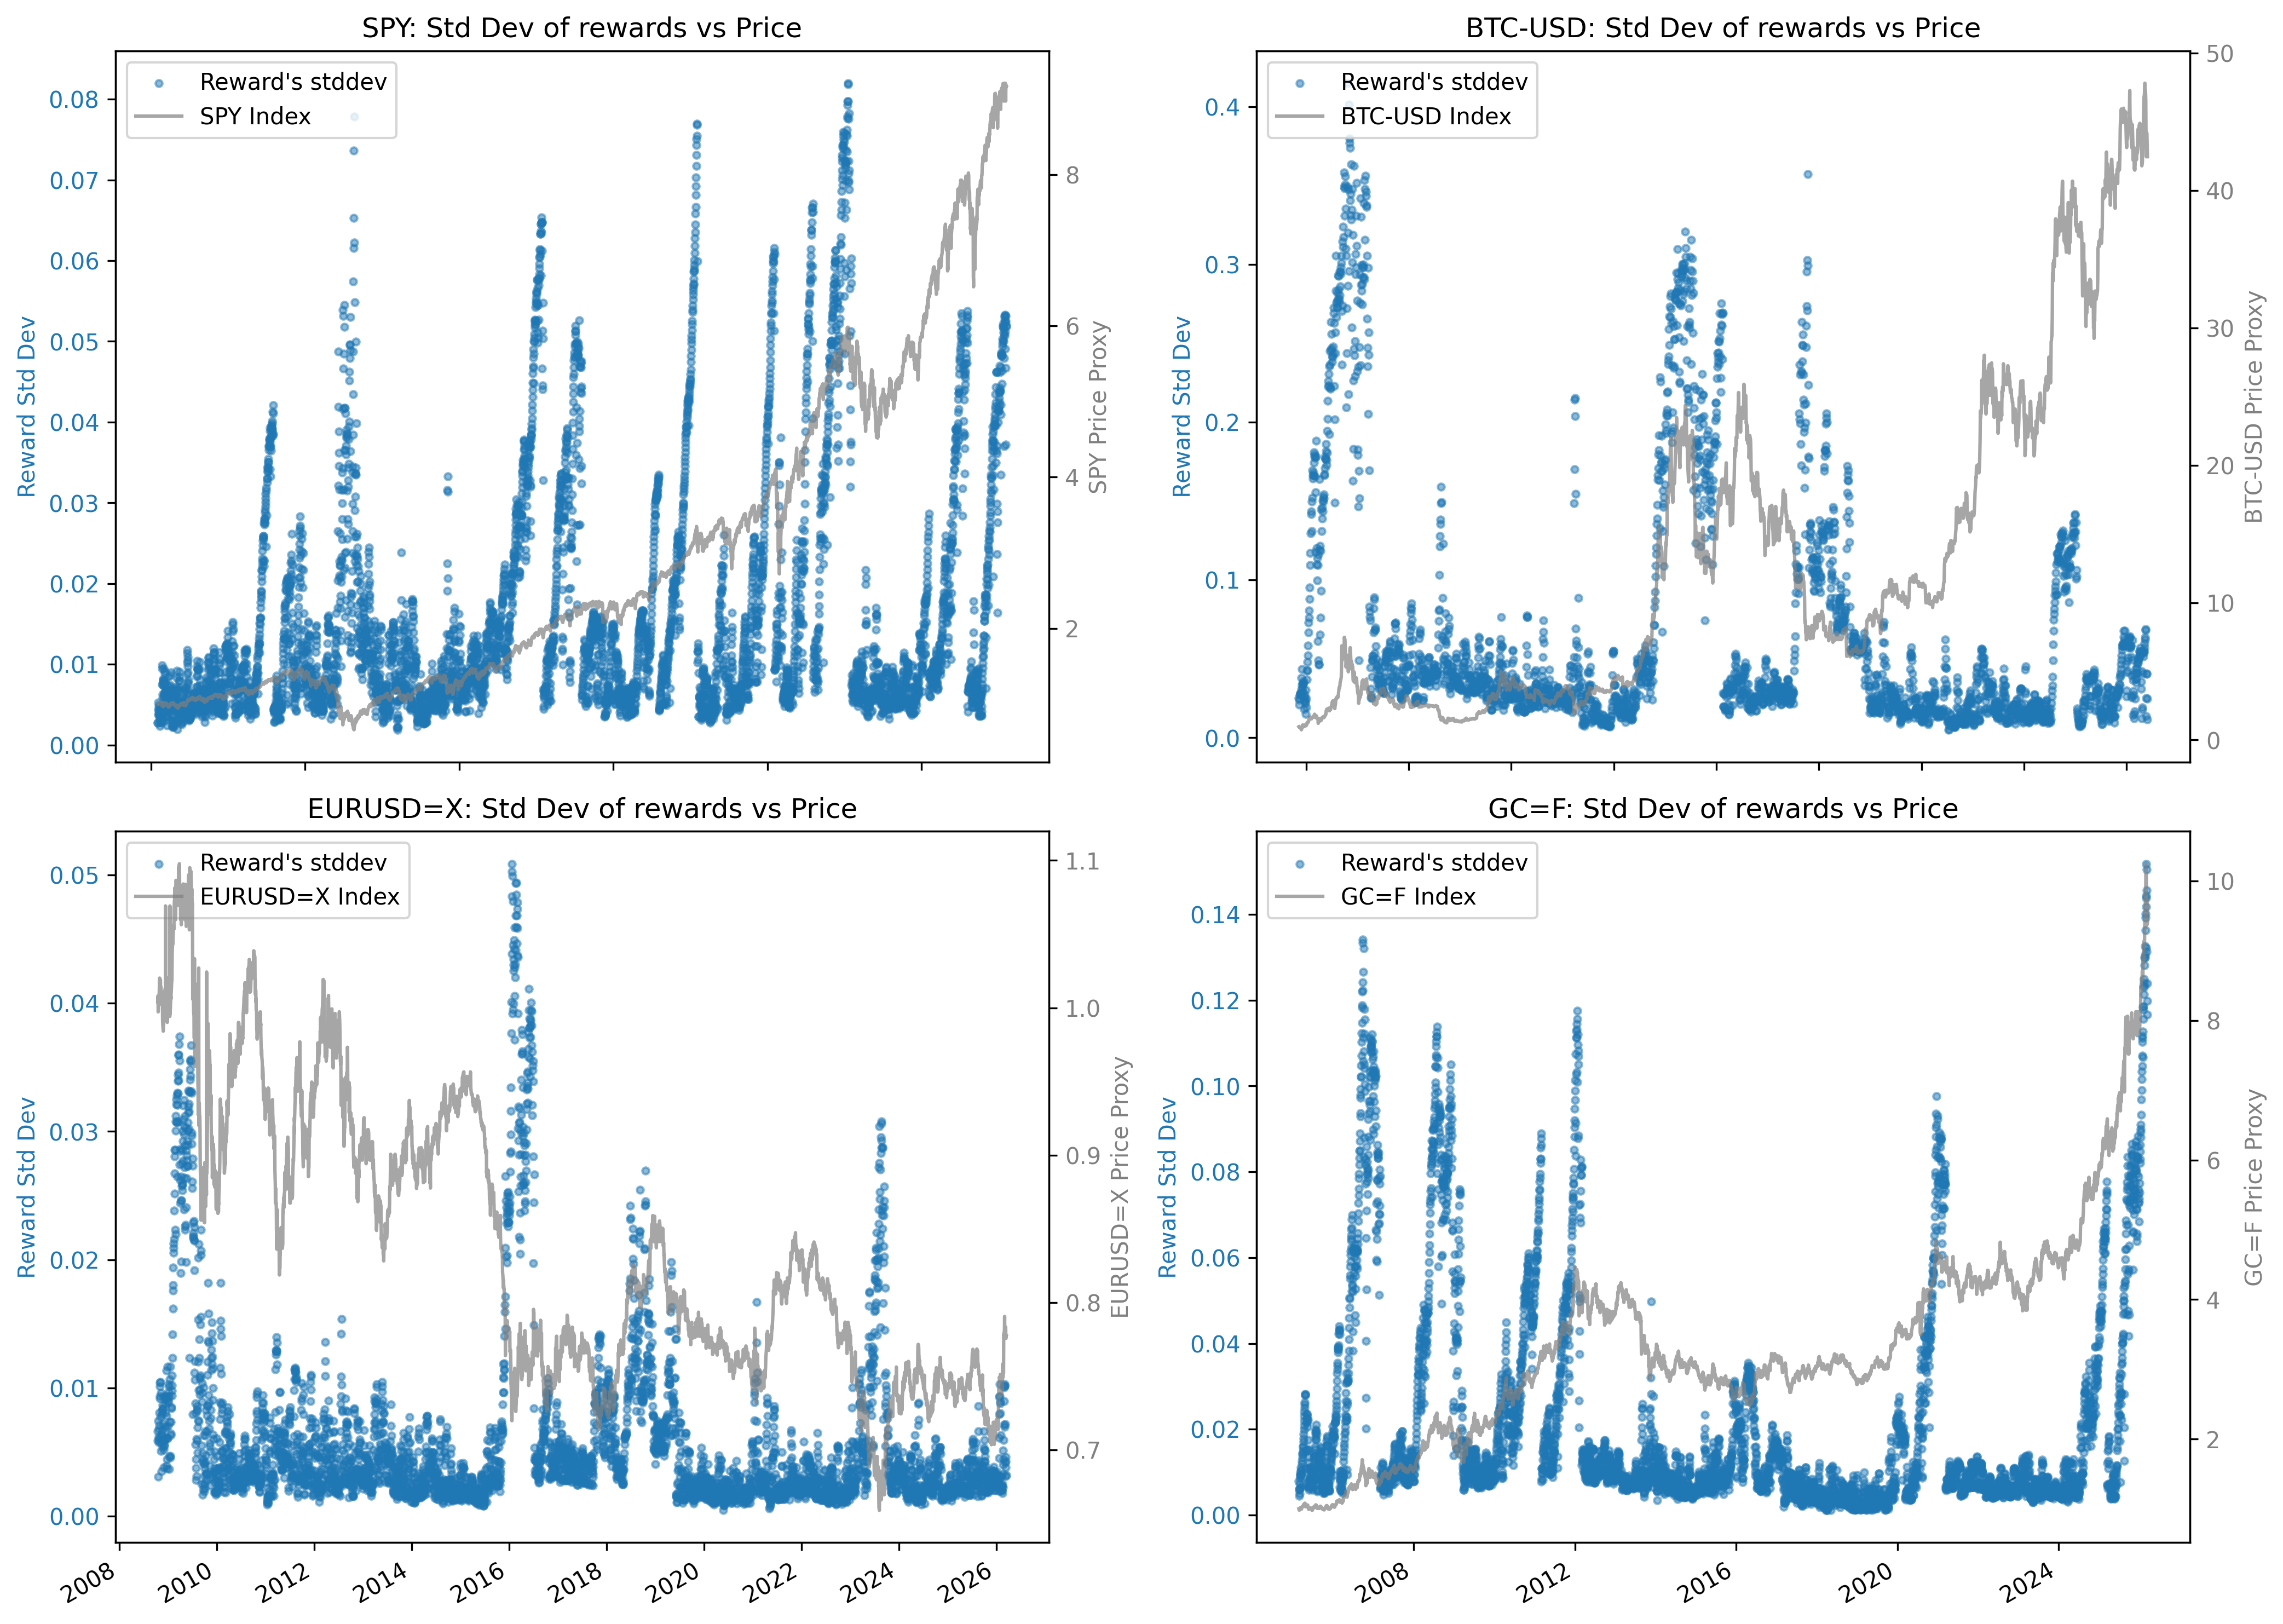
\includegraphics[width=\textwidth]{reward_stddev_grid.png}
    \caption{Cross-sectional standard deviation of the reward signals across the pool of base models for four diverse asset classes (Equities, Cryptocurrency, Sovereign Bonds, and Foreign Exchange). The cumulative return of the underlying asset is overlaid in gray. Across all datasets, periods of market stress or significant drawdowns consistently coincide with a spike in reward standard deviation, indicating heightened disagreement among predictors during highly volatile, non-stationary regimes.}
    \label{fig:reward_stddev}
\end{figure}

\subsection{Impact of Architectural Heterogeneity}
\label{sec:heterogeneity}

To further validate the robustness of our dynamic selection framework and address the imperative of out-of-sample generalizability, we investigate the impact of architectural diversity within the predictor pool. Figure \ref{fig:variance_comparison} illustrates the divergence in predictive dispersion—quantified by the 21-day moving average of the cross-sectional standard deviation of the reward signals—between a strictly homogeneous pool (comprising 50 MLPs differing solely by random seed initialization) and a heterogeneous pool (comprising an equal algorithmic mixture of MLPs, CNNs, and RNNs).

As empirically demonstrated in the figure, expanding the base models into a heterogeneous ensemble substantially and consistently amplifies the cross-sectional variance relative to the baseline aleatoric variation induced by random weight initialization in the homogeneous pool. This heightened dispersion is theoretically intuitive: disparate neural architectures impose distinct inductive biases on the learning process. For instance, RNNs may exhibit superior predictive capacity during strongly autocorrelated trending periods due to their temporal memory mechanisms, whereas CNNs might more effectively extract localized volatility features or short-term structural patterns. 

Crucially, this elevated structural variance actively penalizes naive, static ensemble aggregation. In a highly diverse pool, the inclusion of temporarily maladapted architectures during sudden regime shifts systematically degrades the ensemble's aggregate performance. This dynamic establishes a rigorous, adversarial environment that empirically underscores the fundamental necessity of our proposed methodology: dynamic, context-aware model selection via CMABs is mathematically critical to isolating and exploiting the optimal inductive bias for any localized market regime.

\begin{figure}[htbp]
    \centering
    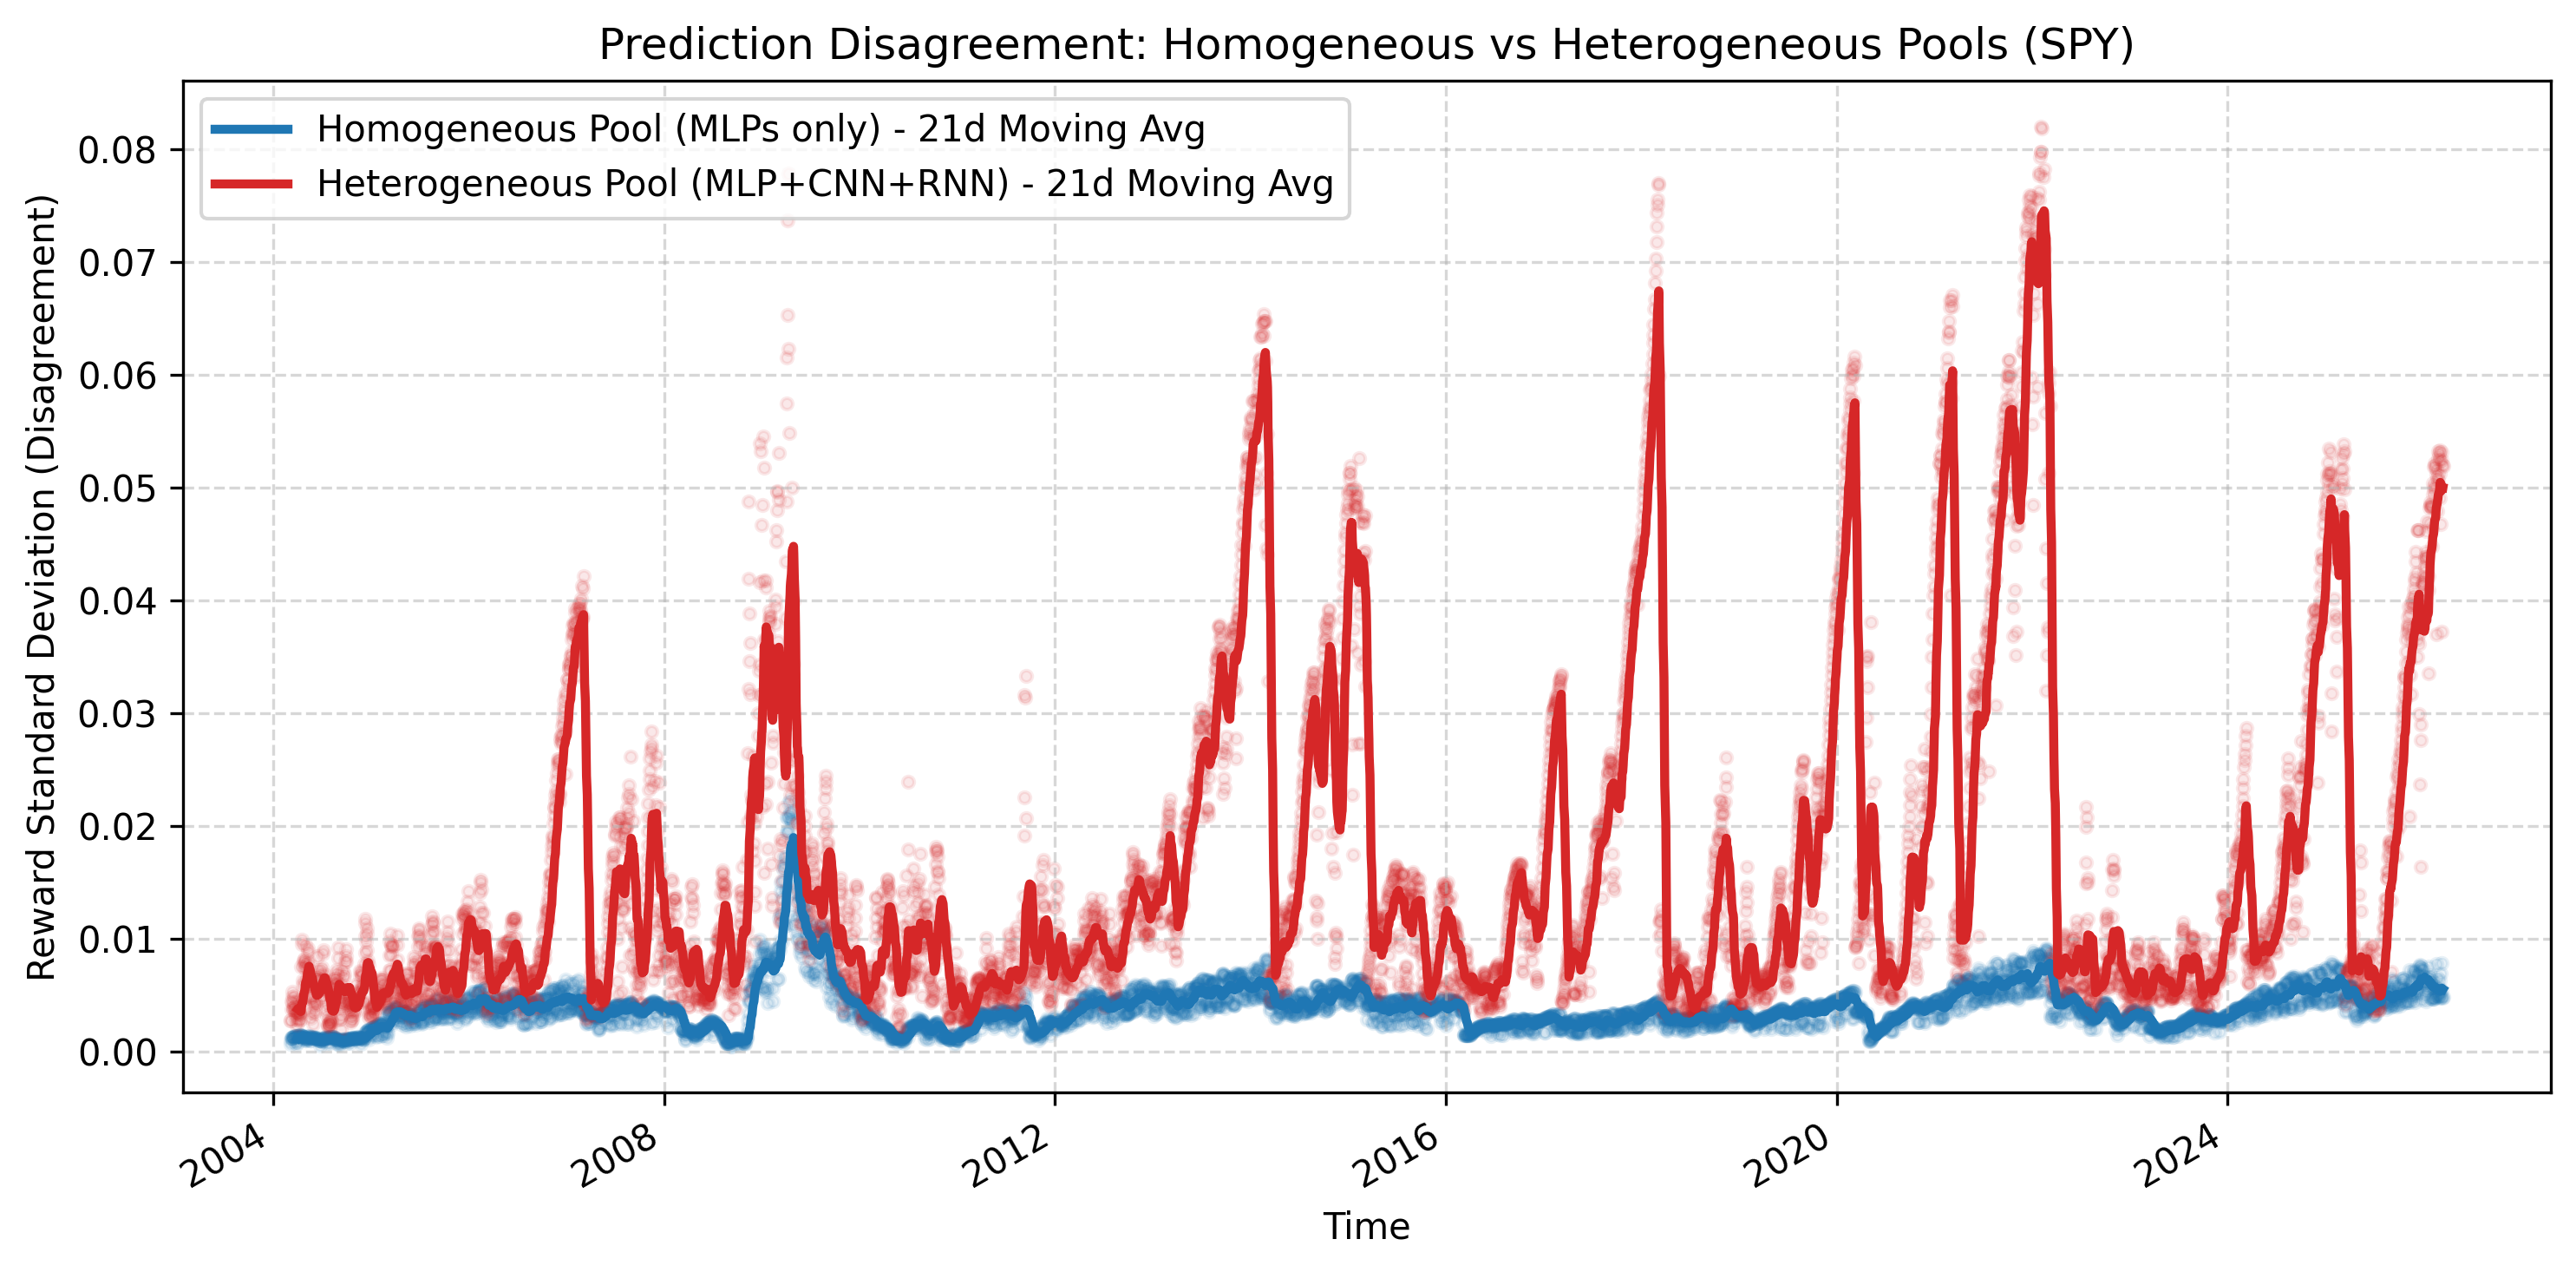
\includegraphics[width=.8\textwidth]{variance_comparison_SPY.png}
    \caption{Comparison of predictive dispersion (represented by the 21-day moving average of the reward standard deviation) between a homogeneous predictor pool (MLPs only) and a heterogeneous pool (MLPs, CNNs, and RNNs) on the SPY dataset. The heterogeneous pool consistently exhibits higher cross-sectional disagreement, reflecting the diverse inductive biases of the constituent architectures. This structural variance actively degrades static ensembling methods, highlighting the necessity for dynamic model selection.}
    \label{fig:variance_comparison}
\end{figure}

\subsection{Context Construction}
\label{sec:context}

We define the context vector $\mathbf{x}_{t,a} \in \mathbb{R}^n$ for each arm $a$ at time $t$ as the sequence of the past $n$ rewards that the specific predictor would have generated had it been selected in the immediately preceding time steps:
\begin{equation}
    \mathbf{x}_{t,a} := \left( R_{t-1,a}, R_{t-2,a}, \dots, R_{t-n,a} \right)^\top.
\end{equation}
This autoregressive state formulation explicitly leverages the short-term momentum inherent in the predictive efficacy of localized models. As empirically validated in Figure \ref{fig:acf_reward_L1}, this persistence in model performance is quantitatively evident; the global mean autocorrelation function of the reward signals exhibits a statistically significant, positive correlation at early lags across the various predictors and asset classes.

\begin{figure}[htbp]
    \centering
    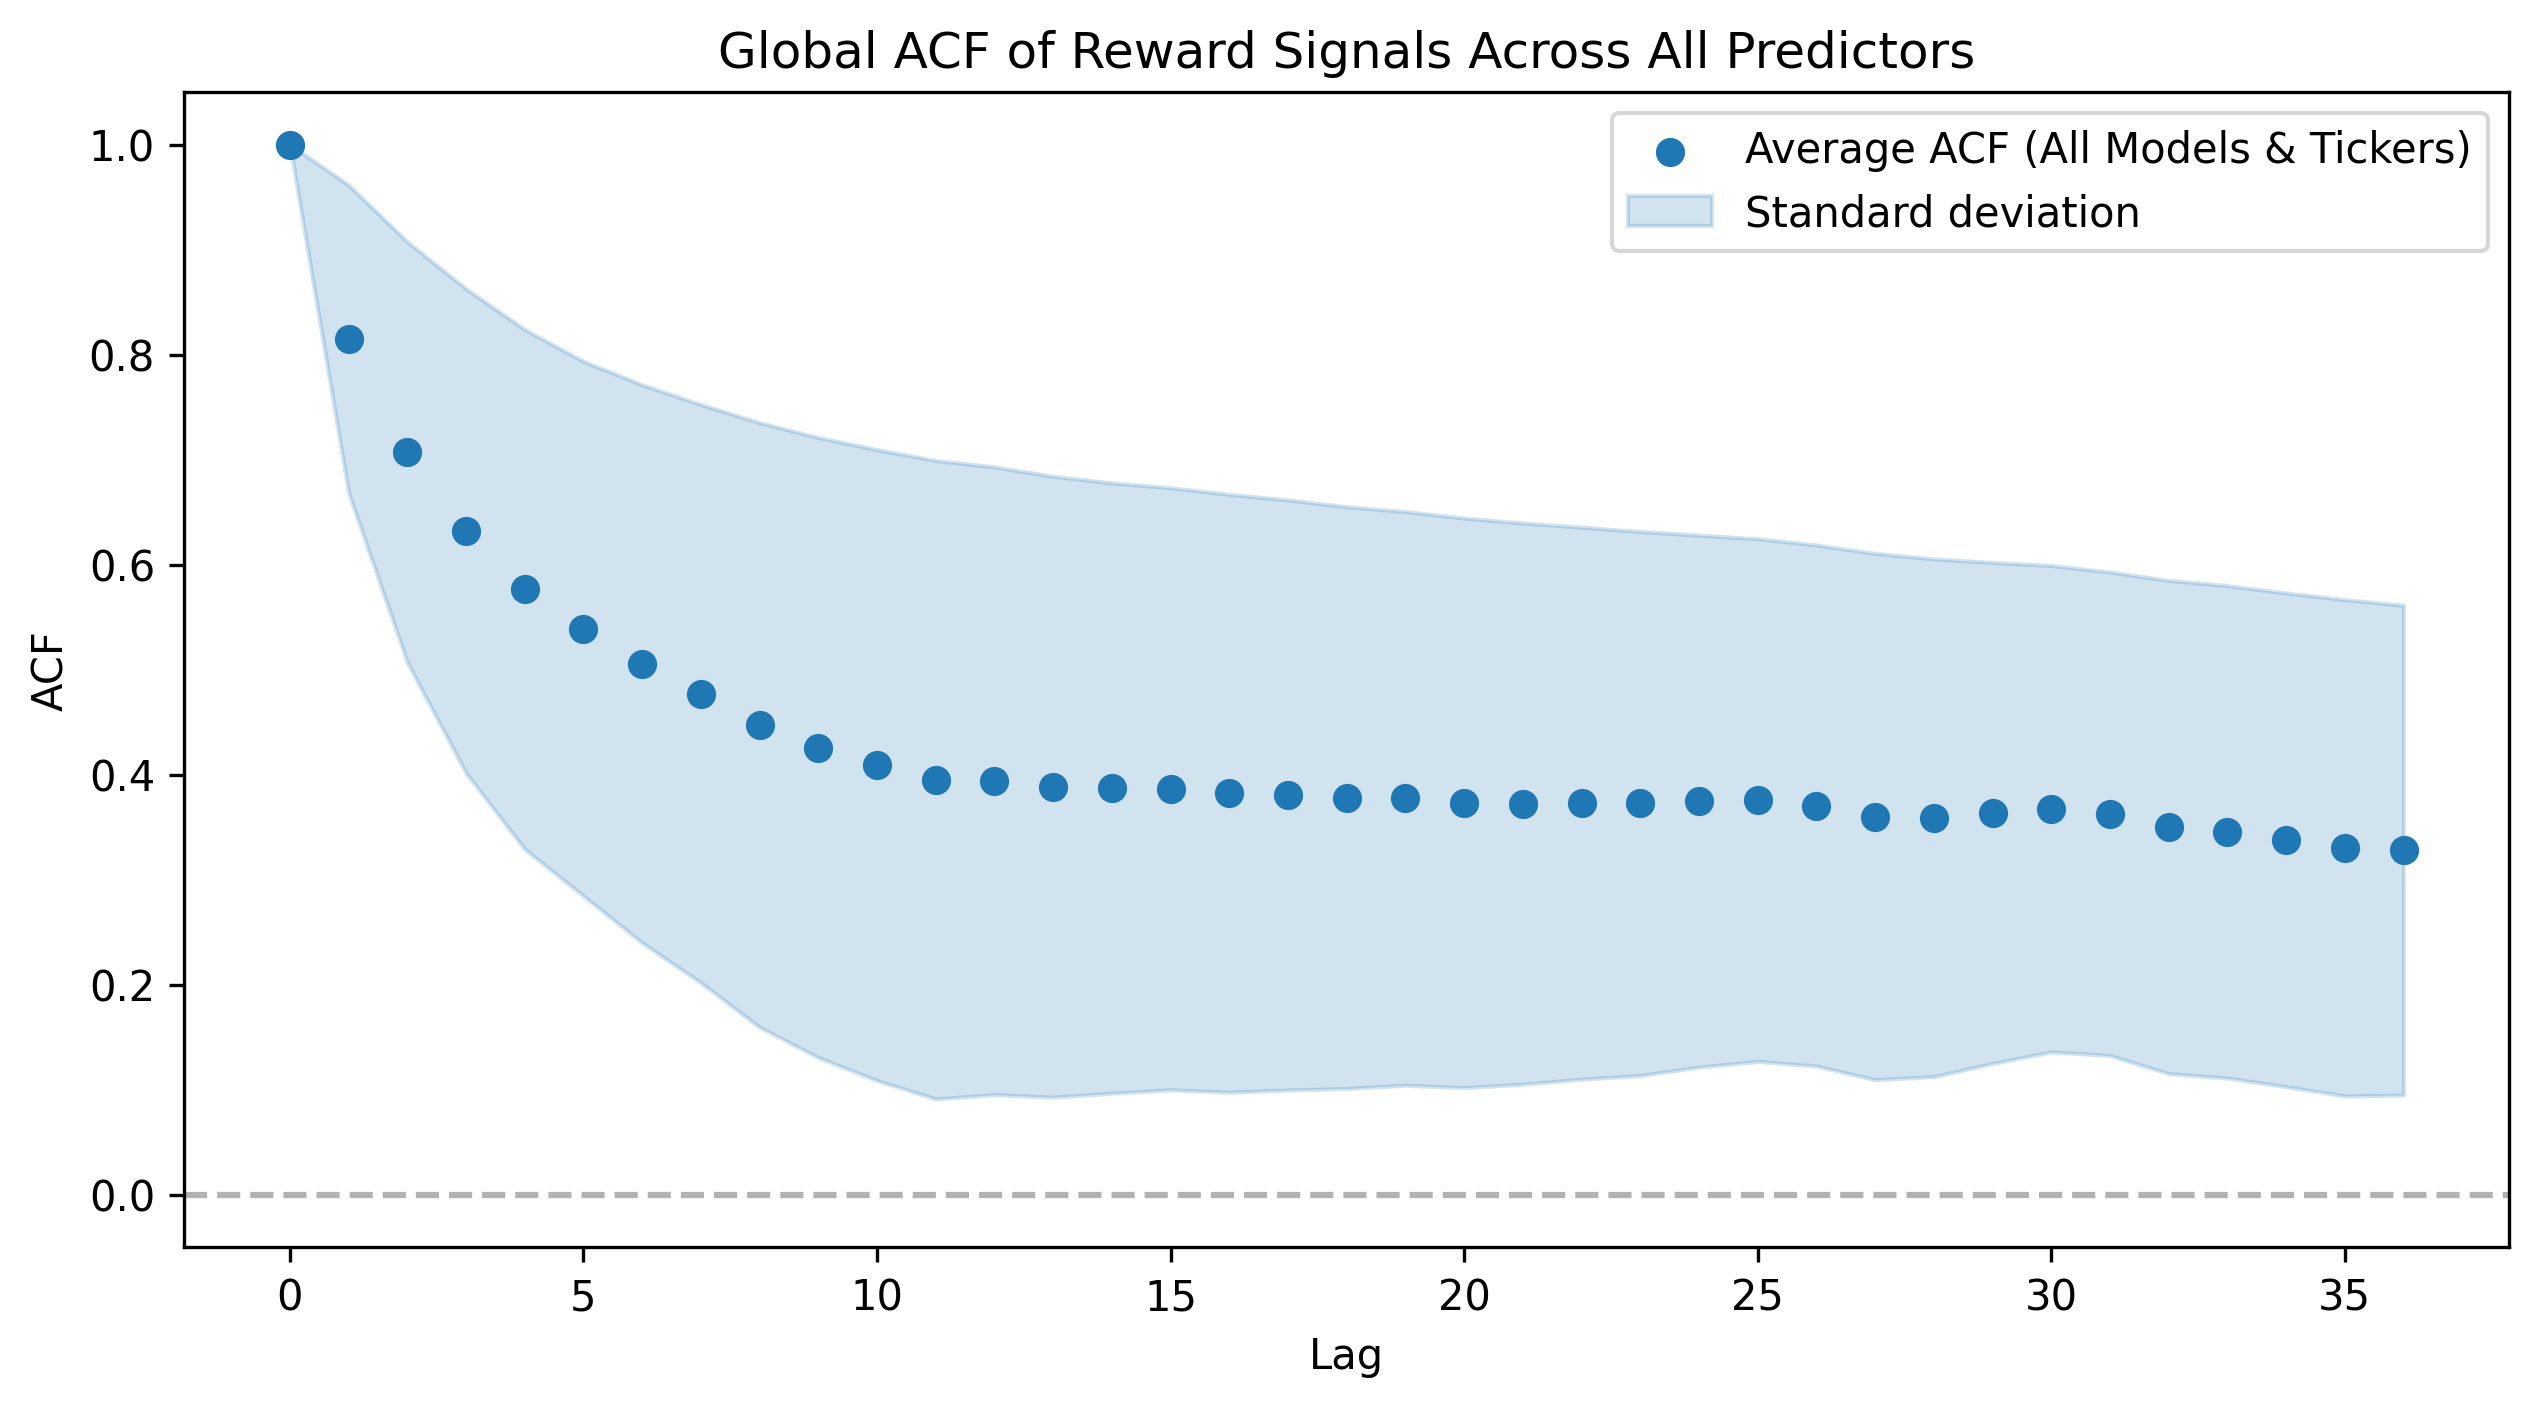
\includegraphics[width=.8\textwidth]{reward_acf_global.png}
    \caption{Global mean autocorrelation function (ACF) of the reward signals, aggregated across all base predictors and all evaluated datasets. The shaded region represents a one-standard-deviation confidence interval. The pronounced positive autocorrelation at early lags demonstrates a short-term persistence in model performance (epistemic momentum) across different asset classes, empirically justifying our autoregressive context construction.}
    \label{fig:acf_reward_L1}
\end{figure}

Furthermore, while contemporary literature emphasizes the integration of risk-aware metrics—such as asset variance or maximum drawdown—into MAB formulations for continuous portfolio selection \cite{huo2017risk}, we omit such market-level risk metrics from our context vector. Because our framework evaluates distinct predictive models on the \emph{same} underlying asset, any market-derived risk metric (e.g., rolling historical volatility) would take an identical numeric value across all arms at a given time step $t$. We note that, in a disjoint (per-arm) linear model such as ours, a shared feature is not automatically non-discriminatory in principle: since each arm learns its own weight vector $\theta_{t,a}$, distinct arms could in principle assign this shared input different coefficients and derive some benefit from it. Our design rationale is instead that such a feature reflects a property of the \emph{asset}, not of the model producing the forecast, and therefore carries no genuinely arm-specific information for the policy to exploit -- so we hypothesized it would offer limited practical benefit for differentiating between models. Rather than relying on this argument alone, we test it directly: Appendix \ref{sec:ablation} reports a controlled ablation appending exactly such a feature to the context, and finds it is not merely uninformative but, for our strongest-performing policy (LinUCB), measurably harmful -- an empirical result that, if anything, strengthens rather than merely confirms our design choice to exclude it.

\subsection{Trading Strategy Formulation}
\label{sec:pred}

The point forecast generated by the greedily selected CMAB arm during the out-of-sample deployment phase is utilized to drive a systematic, long-only directional trading strategy. Let $\hat{y}_t$ denote the forecasted closing price for time $t$ produced by the selected arm, and $y_{t-1}$ represent the last observed closing price. The discrete trading signal, $S_t \in \{0, 1\}$, is formulated as:
\begin{equation}
    S_t = 
    \begin{cases} 
      1, & \text{if } \hat{y}_t > y_{t-1} \\
      0, & \text{otherwise}
    \end{cases}
\end{equation}
When $S_t = 1$, the framework allocates the entirety of the portfolio capital to a long position in the underlying asset. Conversely, when $S_t = 0$ (indicating a forecasted price decline), the portfolio is fully liquidated into a neutral cash position. In accordance with the assumptions outlined in Section \ref{sec:dataset}, this cash position accrues a 0\% risk-free rate of return. For the purposes of this comparative study, transaction costs and slippage are assumed to be zero to isolate the pure predictive edge of the selection mechanism.

To establish a rigorous comparative baseline for evaluating our dynamic CMAB framework, Figure \ref{fig:mean_cum_return} illustrates the cumulative returns of this identical trading strategy when dictated by individual, static base predictors versus a naive, equally weighted ensemble average. The pronounced dispersion among the individual models (gray lines) underscores the substantial financial risk associated with static, single-model selection. While the static ensemble average (orange line) does not necessarily outperform a passive buy-and-hold strategy, it effectively mitigates the idiosyncratic variance of the individual models. Consequently, it serves as a robust, stabilized machine-learning benchmark against which the adaptive CMAB agents can be rigorously evaluated.

\begin{figure}[htbp]
    \centering
    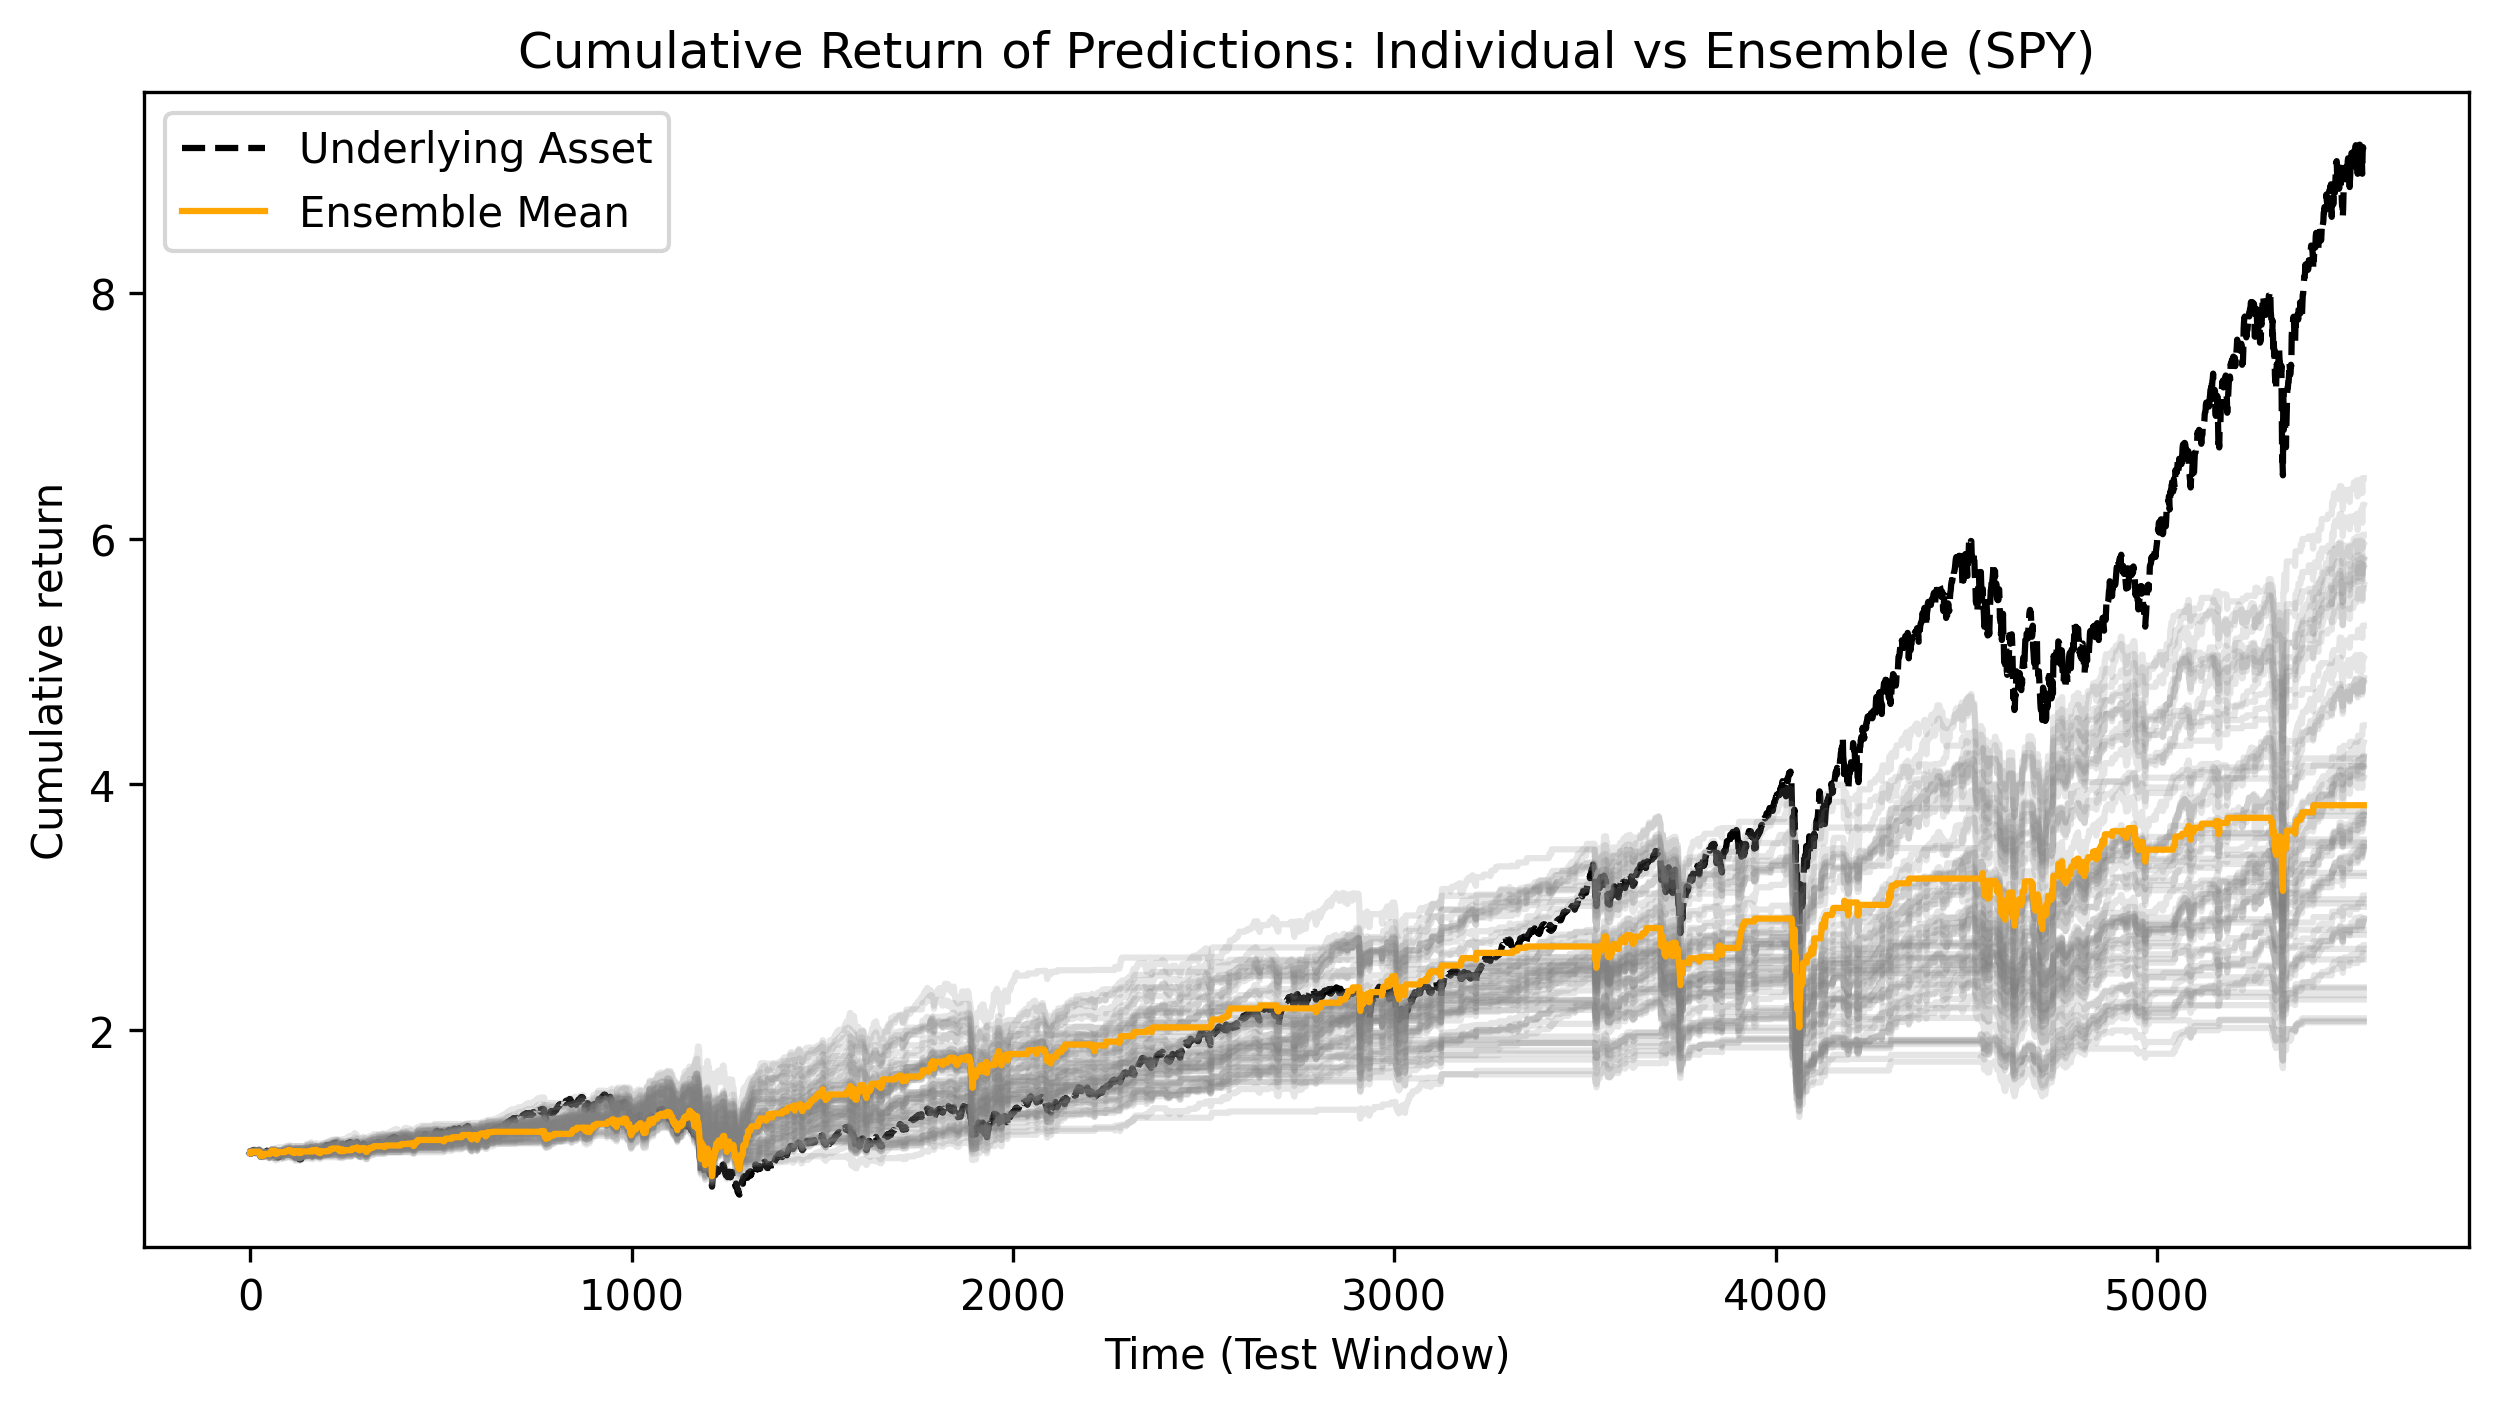
\includegraphics[width=.8\textwidth]{mean_cum_return_rep.png}
    \caption{Cumulative returns of the directional trading strategies derived from individual base predictors (gray) compared to the naive, equally weighted ensemble average (orange) and the underlying buy-and-hold asset return (dashed black). This representative plot (evaluated on the QQQ dataset) highlights the extreme variance in individual model performance. By smoothing this variance, the ensemble average provides a stabilized comparative baseline for our subsequent CMAB evaluations.}
    \label{fig:mean_cum_return}
\end{figure}

\section{Results and Performance Analysis}
\label{sec:results}

This section evaluates the out-of-sample performance of the directional trading strategies formalized in Section \ref{sec:pred}, which are driven by the deterministic forecasts generated by the CMAB frameworks during their greedy exploitation phase. To rigorously validate the generalizability of our approach across distinct market microstructures and volatility regimes, our empirical evaluation spans five diverse asset classes: SPY (Broad Market Equities), BTC-USD (Cryptocurrency), TLT (Sovereign Bonds), EURUSD=X (Foreign Exchange), and GC=F (Commodities). 

Throughout this section, while comprehensive aggregated metrics are reported for all evaluated assets, we frequently highlight the SPY dataset as a representative benchmark to visualize the localized, step-by-step mechanics of the dynamic model selection process.

\subsection{Generalizability and Multi-Policy Comparison}

Table \ref{tab:main_results} presents a comprehensive summary of the out-of-sample performance metrics across all evaluated datasets. We rigorously benchmarked three distinct CMAB exploration policies (Softmax optimized via SGA, LinUCB, and Thompson Sampling) against the standard static Ensemble Average. Furthermore, to isolate the impact of structural variance, these policies were evaluated across two distinct environments: a homogeneous predictor pool (comprising exclusively identically parameterized MLPs) and a heterogeneous pool (comprising a diverse mixture of MLPs, CNNs, and RNNs).

The empirical findings clearly demonstrate that the dynamic CMAB selection framework generalizes effectively across fundamentally different asset classes and market microstructures. Across the majority of the evaluated time series, the deterministic trading strategies driven by the CMAB frameworks outperformed the naive ensemble average in both absolute annualized returns and risk-adjusted metrics (Sharpe Ratio). 

Crucially, the experimental results reveal a pronounced performance hierarchy among the bandit policies themselves, directly underscoring the critical importance of robust exploration mechanisms. While the gradient-updated Softmax policy generally improves upon the static ensemble baseline, it is consistently outperformed by contextual MAB methods that explicitly quantify and manage epistemic uncertainty. As detailed in Table \ref{tab:main_results}, the Upper Confidence Bound (LinUCB, denoted as UCB) policy emerges as the point-estimate leader. Across almost all asset classes (BTC-USD, EURUSD=X, GC=F, and SPY), UCB achieves the highest Annualized Returns and Sharpe Ratios, consistent with explicitly bounding exploration uncertainty being advantageous in non-stationary financial environments. We stress, however, that this ranking is a point-estimate comparison: as reported in Section \ref{sec:significance}, none of the 30 individual CMAB-vs-ensemble gaps underlying this table remain statistically significant after correcting for multiple comparisons, so UCB's lead should be read as a consistent directional pattern across asset classes rather than a per-asset statistically confirmed effect.

However, for the sake of transparency, it is important to note that the dynamic CMAB framework does not yield universal outperformance across all conceivable market conditions. As detailed in Table \ref{tab:main_results}, the TLT dataset (Sovereign Bonds) represents a notable exception where the static Ensemble Average marginally outperformed the contextual bandit policies in both environments. This divergence likely stems from the distinct market microstructure of sovereign debt. Unlike equities or crypto, bond prices are heavily anchored to exogenous macroeconomic factors—specifically, central bank interest rate policies and rigid macroeconomic cycles—rather than the localized, short-term autoregressive price momentum that our context vectors are explicitly designed to exploit. In regimes where such structural variance is lower and external macro shocks dominate the price action, the aggressive smoothing properties of a static ensemble may temporarily yield a more stable, albeit conservative, predictive baseline.

A critical secondary objective of this study was to evaluate the performance differential between the homogeneous and heterogeneous predictor pools. The inclusion of CNNs and RNNs inherently introduced structural variance into the prediction space, though its net impact on aggregate performance varied by asset class. In specific markets, such as Commodities (GC=F), the empirical data perfectly validates our core hypothesis: the architectural heterogeneity acted as a severe penalty for the static Ensemble Average (driving its Sharpe Ratio down from 0.34 to 0.24), whereas the explicitly exploratory UCB policy actively thrived on this diversity, improving its Sharpe Ratio from 0.54 to 0.62. While this divergence is most spectacular in the GC=F dataset, it effectively crystallizes the fundamental value proposition of the proposed framework: UCB possesses the capacity to safely navigate and exploit diverse inductive biases in chaotic regimes where static averaging breaks down.


\begin{figure}[htbp]
    \centering
    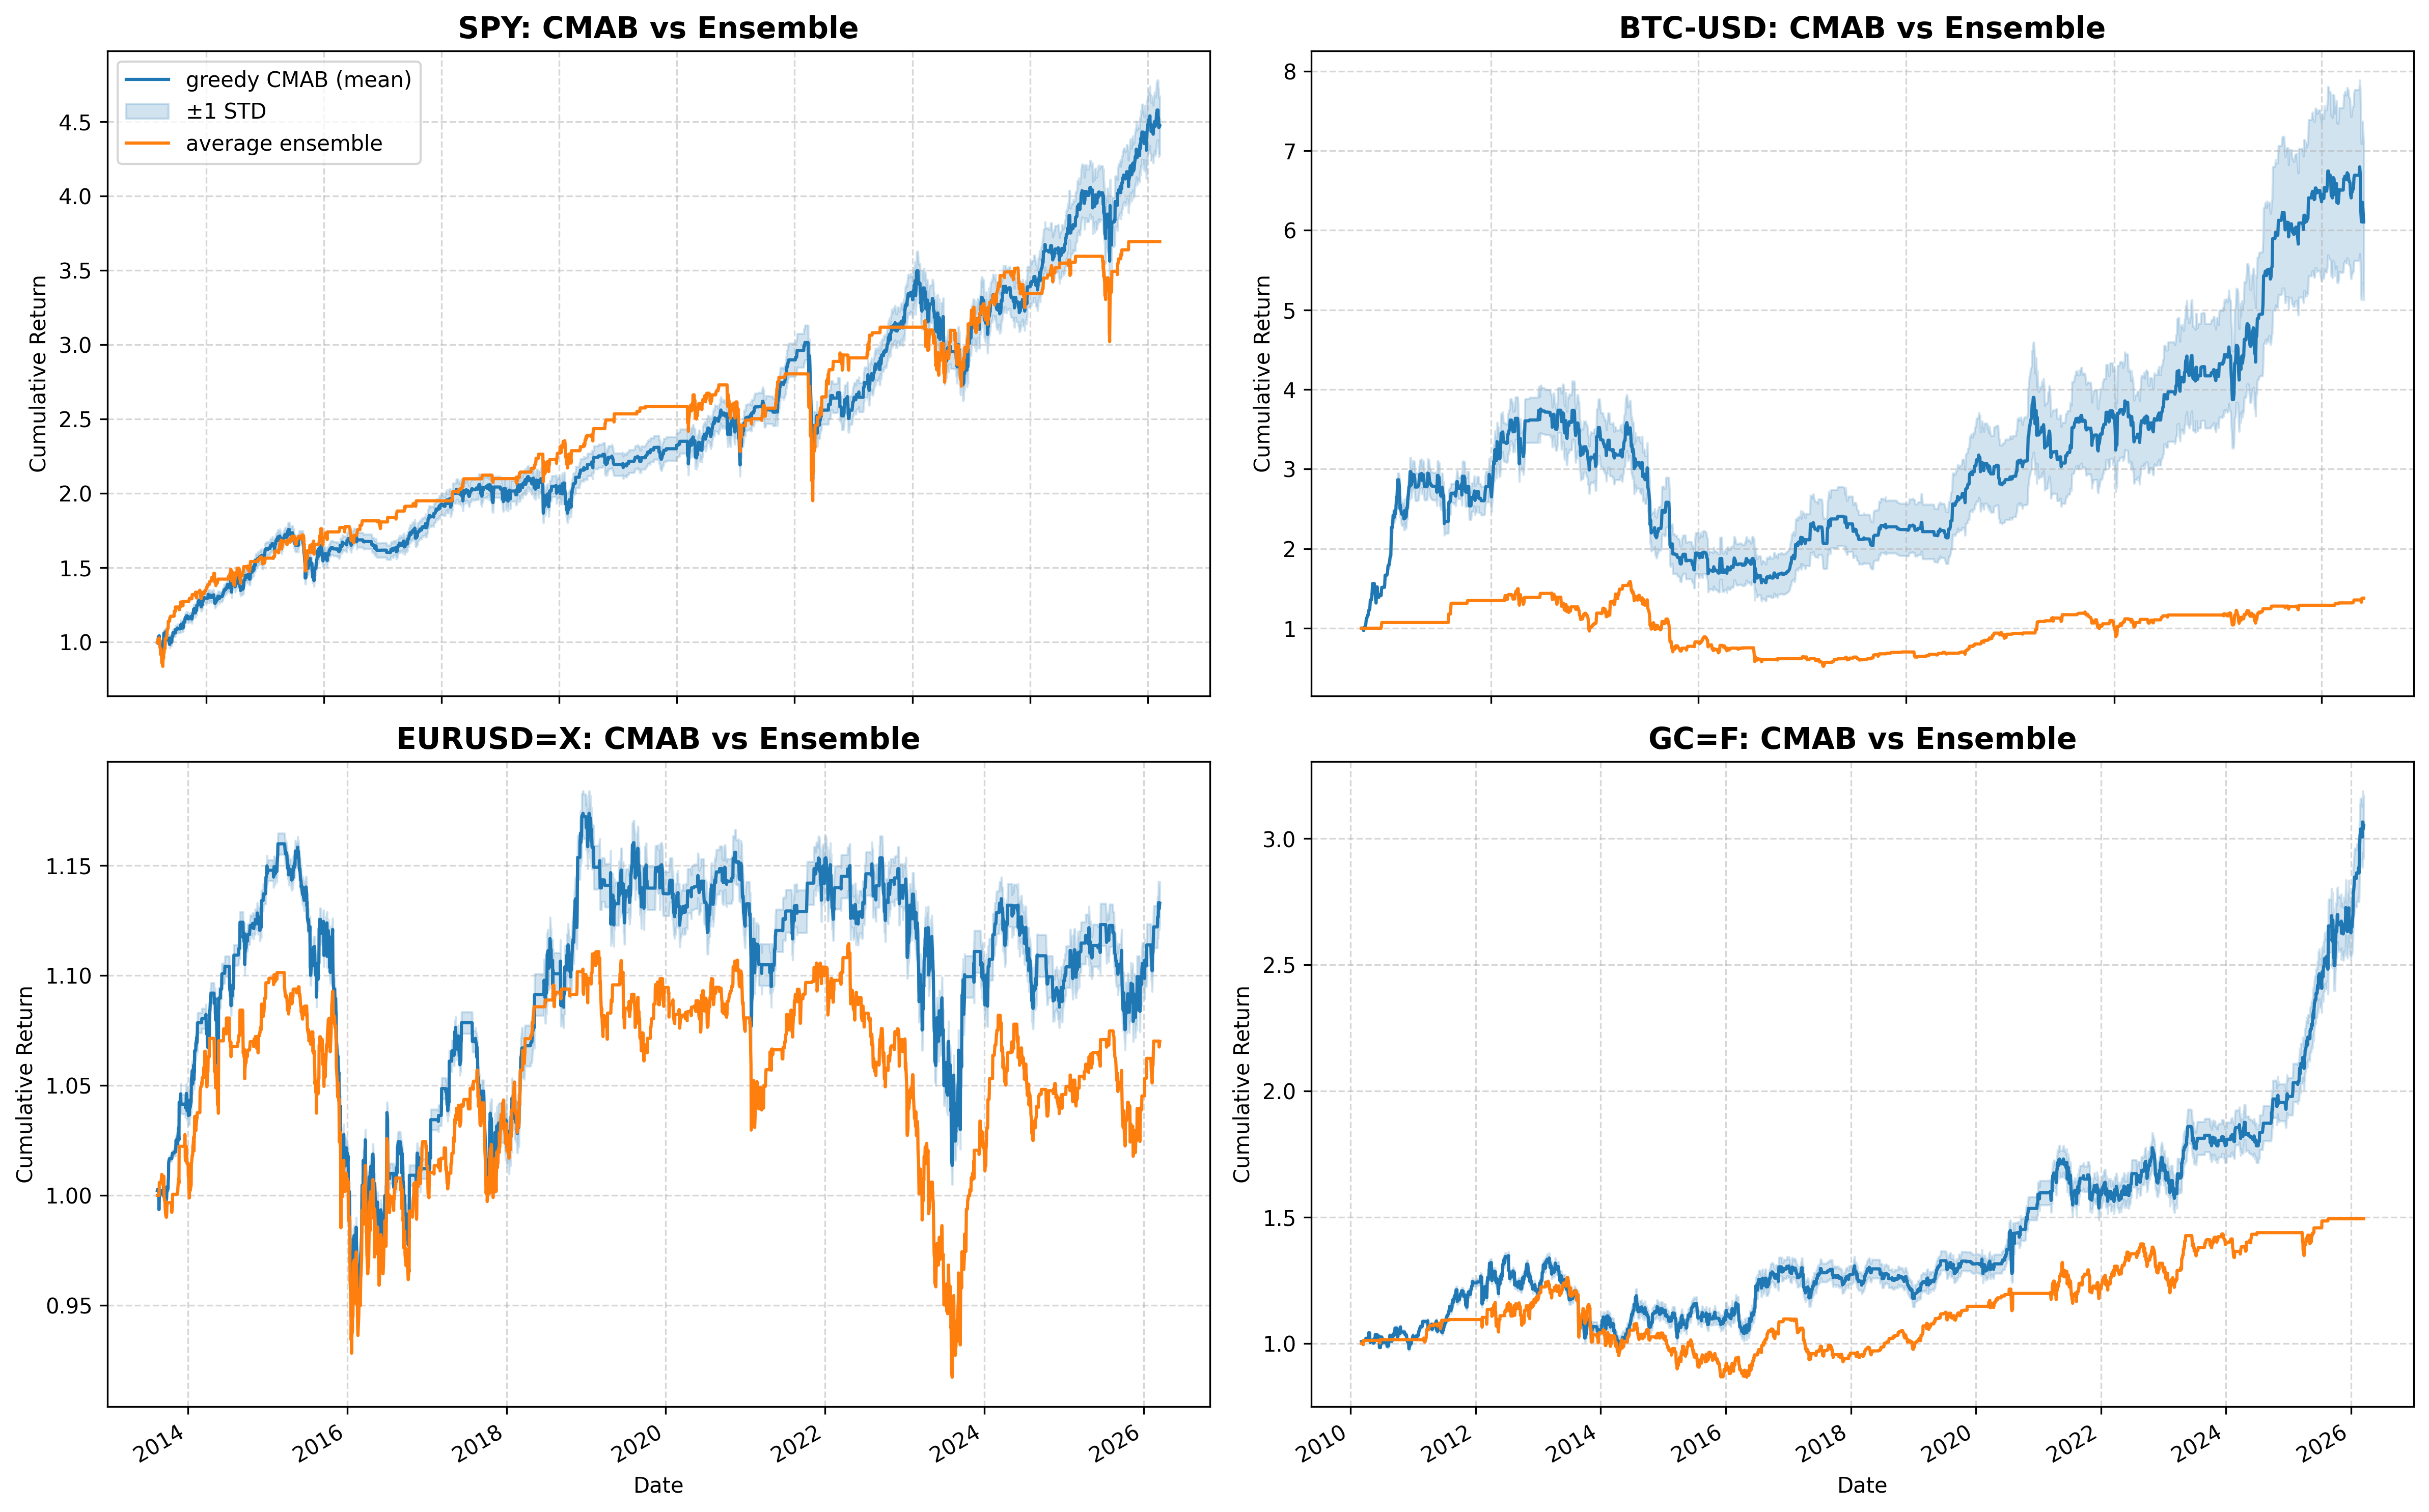
\includegraphics[width=\textwidth]{multi_run_grid_plot1.png}
    \caption{Out-of-sample cumulative returns of the deterministic CMAB strategy compared to the average ensemble baseline across four distinct asset classes. The solid lines represent the mean cumulative Net Asset Value (NAV) across multiple training seeds, while the shaded regions denote a $\pm 1$ standard deviation confidence interval. The results consistently demonstrate the CMAB framework's ability to achieve superior compounded returns while effectively managing the structural variance introduced by the diverse predictor pool.}
    \label{fig:performance_grid}
\end{figure}


\begin{sidewaystable}[htbp]
    \centering
    \caption{Out-of-sample performance metrics across five diverse asset classes. The underlying data spans from January 2000 to March 2026, though out-of-sample testing begins only after the initial four-year walk-forward training window (Section \ref{sec:dataset}), i.e.\ from approximately 2004 onward. All metrics are calculated using a daily return frequency. The Sharpe Ratio is annualized, assuming 252 trading days per year and a risk-free rate of 0\%. Maximum Drawdown (MDD) represents the largest peak-to-trough drop in the cumulative return curve.}
    \label{tab:main_results}
    
    
    \setlength{\tabcolsep}{3pt} 
    \scriptsize 
    
    \begin{tabular}{@{} ll rrrr rrrr rrrr @{}}
    \toprule
     & & \multicolumn{4}{c}{\textbf{Annualized Return}} & \multicolumn{4}{c}{\textbf{Sharpe Ratio}} & \multicolumn{4}{c}{\textbf{Max Drawdown}} \\
     \cmidrule(lr){3-6} \cmidrule(lr){7-10} \cmidrule(lr){11-14}
    \textbf{Ticker} & \textbf{Architecture} & Ens & Softmax & UCB & Thomp & Ens & Softmax & UCB & Thomp & Ens & Softmax & UCB & Thomp \\
    \midrule
    \multirow{2}{*}{\textbf{BTC}} & Heterogeneous & 0.05 & 0.19 & \textbf{0.29} & 0.15 & 0.16 & 0.48 & \textbf{0.80} & 0.39 & -0.67 & \textbf{-0.55} & -0.60 & -0.72 \\
     & Homogeneous & 0.07 & 0.15 & \textbf{0.30} & 0.25 & 0.19 & 0.40 & \textbf{0.81} & 0.69 & -0.50 & -0.53 & \textbf{-0.47} & -0.56 \\
    \midrule
    \multirow{2}{*}{\textbf{EURUSD}} & Heterogeneous & 0.01 & 0.00 & \textbf{0.01} & 0.00 & 0.09 & 0.08 & \textbf{0.16} & 0.07 & \textbf{-0.18} & -0.20 & -0.19 & -0.20 \\
     & Homogeneous & -0.01 & 0.00 & \textbf{-0.00} & -0.00 & -0.16 & \textbf{0.08} & -0.03 & -0.08 & -0.26 & \textbf{-0.21} & -0.21 & -0.25 \\
    \midrule
    \multirow{2}{*}{\textbf{GC=F}} & Heterogeneous & 0.03 & 0.03 & \textbf{0.07} & 0.07 & 0.24 & 0.24 & \textbf{0.62} & 0.61 & -0.31 & -0.36 & -0.27 & \textbf{-0.22} \\
     & Homogeneous & 0.04 & 0.05 & \textbf{0.06} & 0.06 & 0.34 & 0.39 & \textbf{0.54} & 0.47 & \textbf{-0.24} & -0.27 & -0.34 & -0.28 \\
    \midrule
    \multirow{2}{*}{\textbf{SPY}} & Heterogeneous & 0.08 & 0.08 & \textbf{0.09} & 0.07 & 0.61 & 0.56 & \textbf{0.66} & 0.48 & \textbf{-0.30} & -0.30 & -0.30 & -0.32 \\
     & Homogeneous & 0.09 & 0.09 & \textbf{0.10} & 0.09 & 0.64 & 0.66 & \textbf{0.69} & 0.65 & -0.36 & -0.34 & \textbf{-0.31} & -0.34 \\
    \midrule
    \multirow{2}{*}{\textbf{TLT}} & Heterogeneous & \textbf{0.04} & 0.01 & 0.02 & 0.04 & \textbf{0.38} & 0.11 & 0.20 & 0.33 & -0.29 & -0.30 & -0.36 & \textbf{-0.23} \\
     & Homogeneous & \textbf{0.03} & 0.01 & 0.02 & 0.03 & \textbf{0.27} & 0.09 & 0.20 & 0.27 & -0.27 & -0.30 & -0.27 & \textbf{-0.25} \\
    \bottomrule
    \end{tabular}
\end{sidewaystable}

\subsection{Mechanics of Dynamic Selection}
\label{sec:dynamic}

The fundamental theoretical advantage of formulating model selection as a CMAB problem lies in its structural capacity to dynamically adapt to non-stationary financial regimes. Static ensemble methods, by definition, impose rigid aggregation weights across the predictor pool regardless of the current market context. While this heuristic provides global variance reduction, it structurally limits the strategy's ability to exploit isolated, highly localized predictive superiority. 

To empirically visualize these adaptive mechanics, we examine a representative execution of the CMAB operating on the SPY dataset. Figure \ref{fig:color-by-arm} explicitly maps the internal routing of the algorithm, utilizing a distinct color mapping to highlight the specific base predictor (arm) chosen by the policy's deterministic exploitation mechanism at each out-of-sample time step $t$.

\begin{figure}[htbp]
    \centering
    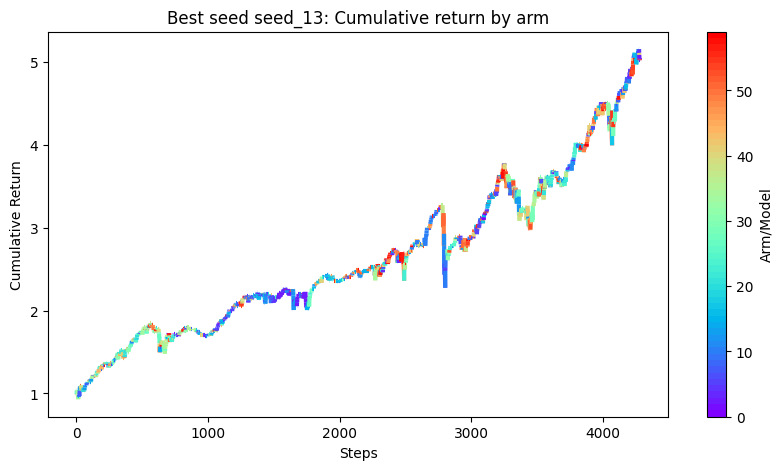
\includegraphics[width=0.8\textwidth]{color_by_arm.png}
    \caption{Cumulative return trajectory of the CMAB strategy on the SPY dataset, color-coded by the active base predictor. Each distinct color segment corresponds to the specific arm selected by the greedy exploitation policy at time $t$. The high frequency of color transitions visually demonstrates the bandit's continuous adaptation to shifting, localized market regimes.}
    \label{fig:color-by-arm}
\end{figure}

The visualization reveals a high frequency of state transitions in arm selection, demonstrating that the bandit actively shifts its preference in direct response to the autoregressive context vectors (i.e., short-term epistemic momentum). By continuously promoting and demoting individual models as their predictive efficacy fluctuates in and out of phase with the underlying asset's structural drift, the CMAB effectively operates as a dynamic momentum filter for the predictor pool. This explicit routing mechanism mathematically explains the outperformance observed previously in Figure \ref{fig:performance_grid}: rather than permitting temporarily maladapted models to systematically dilute the aggregate forecast—a fundamental flaw of static ensembling—the contextual bandit seamlessly isolates and deploys the optimal inductive bias for the immediate, localized market regime.

\subsection{Robustness Analysis: Synthetic Placebo Test}
\label{sec:synthetic_data}

A fundamental econometric concern when applying highly parameterized deep learning architectures to financial time series is the risk of overfitting to stochastic noise, thereby generating spurious predictability. To rigorously evaluate whether our proposed CMAB framework genuinely isolates exploitable market inefficiencies—rather than merely memorizing random localized patterns—we conducted a simulation-based robustness check via a synthetic placebo test.

We generated a synthetic price trajectory using a GARCH(1,1) process, calibrated to emulate the broad statistical moments of the S\&P 500 index (an annualized volatility of approximately 16\% and a constant annualized drift of 8.5\%). While this stochastic process correctly simulates realistic financial phenomena such as volatility clustering and structural drift, its directional returns are strictly driven by unforecastable Gaussian noise, fundamentally lacking the complex structural inefficiencies present in empirical market data. Unless otherwise noted, the results reported in this subsection reflect a single synthetic realization (fixed generator seed); characterizing realization-to-realization dispersion for this placebo test is left to future work, alongside the full predictor-pool retraining pass discussed in Section \ref{sec:conclusion}. We then trained our heterogeneous pool of base predictors on this dataset and applied the UCB contextual selection policy.

The empirical results on the synthetic data, illustrated in Figure \ref{fig:synthetic_test}, perfectly corroborate our theoretical expectations. Because the underlying dataset contained only a static upward drift buried in pure noise, the equally weighted Ensemble Mean effectively captured the baseline market beta. Conversely, the explicitly exploratory CMAB policy, attempting to dynamically adapt to non-existent regime shifts, succumbed to structural whipsaw and systematically failed to outperform the naive baseline. 

\begin{figure}[htbp]
    \centering
    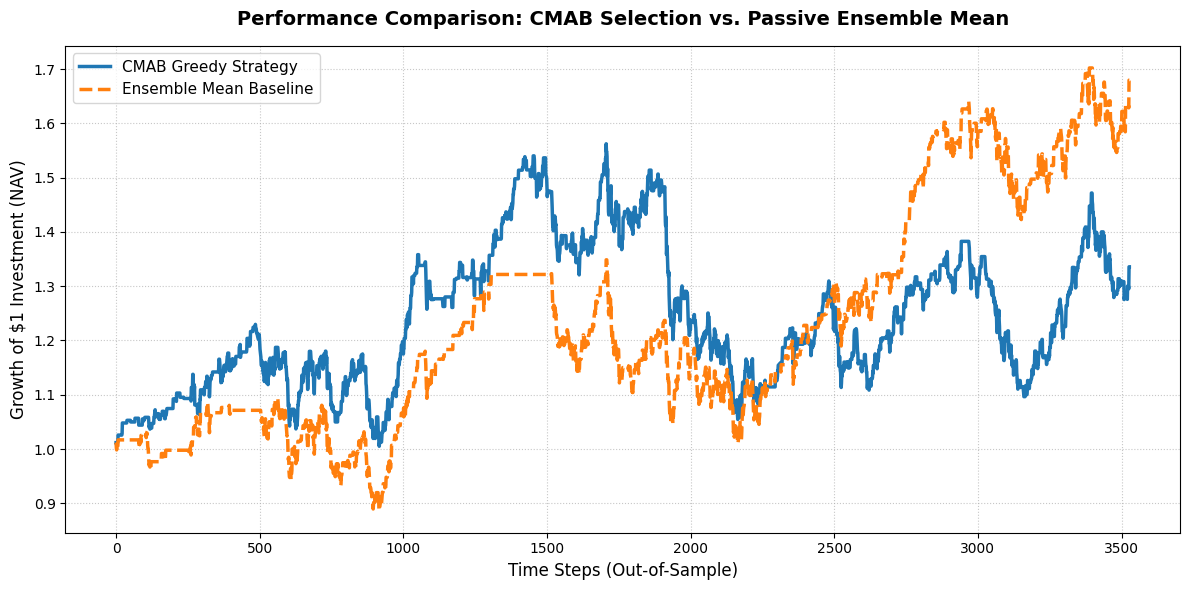
\includegraphics[width=0.8\textwidth]{synthetic_data_comparison.png}
    \caption{Out-of-sample cumulative returns of the deterministic CMAB strategy (UCB) compared to the average ensemble baseline on a synthetic GARCH(1,1) price series. The underlying asset features realistic volatility clustering and constant upward drift but strictly lacks exploitable directional predictability. Consequently, the dynamic CMAB policy is penalized by the noise, failing to outperform the static ensemble mean.}
    \label{fig:synthetic_test}
\end{figure}

This placebo test provides compelling evidence that the CMAB framework does not hallucinate predictive alpha from pure noise or volatility clusters. Instead, it confirms that the outperformance observed on the real-world empirical datasets (e.g., SPY, BTC-USD, GC=F) is strictly driven by the routing mechanism successfully isolating and exploiting genuine, non-stationary market predictability.

\subsection{Statistical Significance of CMAB vs.\ Static Ensemble}
\label{sec:significance}

The point-estimate gaps reported in Table \ref{tab:main_results} do not, by themselves, establish that the CMAB-greedy strategy's advantage over the static ensemble baseline is statistically distinguishable from zero. To address this directly, we apply a paired Diebold-Mariano test \cite{diebold1995comparing} to the daily return differential (CMAB-greedy minus static ensemble) for each of the 30 configurations underlying Table \ref{tab:main_results}, using a Newey-West/Bartlett-kernel HAC long-run variance estimate \cite{newey1987simple} with automatic bandwidth selection and the Harvey-Leybourne-Newbold small-sample correction \cite{harvey1997testing}. Because the 25 per-seed return columns for a given configuration share an identical market realization and an identical deterministic baseline -- and are therefore not independent replicates -- we run one primary test per configuration on the cross-seed-mean daily return, the same aggregation Table \ref{tab:main_results}'s point estimates already use, rather than treating each seed as an independent comparison. We additionally report a circular moving-block bootstrap 95\% confidence interval (10,000 replicates) for the Sharpe-ratio difference. Recognizing that the 30 configurations constitute a family for multiple-testing purposes, we apply both the Holm procedure (family-wise error rate) \cite{holm1979simple} and Benjamini-Hochberg (false discovery rate) correction \cite{benjamini1995controlling} at $\alpha=0.05$ across the 30 primary $p$-values.

Table \ref{tab:significance} reports the results. \textbf{No configuration remains significant after either the Holm or the Benjamini-Hochberg correction at $\alpha=0.05$.} Only one configuration (GC=F, Thompson Sampling, heterogeneous pool) has a raw, uncorrected $p<0.05$ ($p=0.018$), but its Holm-corrected value is $p=0.551$. Two configurations -- BTC-USD/Thompson/homogeneous and GC=F/Thompson/heterogeneous -- have a bootstrap Sharpe-difference 95\% confidence interval that excludes zero, both favoring the CMAB strategy; these use a different (percentile-bootstrap) inferential procedure than the DM test and are not corrected for multiplicity, so we report them descriptively rather than as confirmed effects.

Twenty of the 30 point estimates favor the CMAB strategy (positive mean-return differential); the ten that do not are concentrated in TLT, consistent with the qualitative exception already noted in Section \ref{sec:results}. We interpret the overall pattern as a directionally consistent but individually modest edge per configuration: with $n$ ranging from 1,764 (BTC-USD) to 4,284 (SPY) daily out-of-sample observations per configuration, and daily strategy returns that are themselves serially correlated (motivating the HAC correction in the first place), a Sharpe-ratio gap of the magnitude reported in Table \ref{tab:main_results} does not, on its own, clear a conservative, multiplicity-corrected significance bar. This tempers -- without invalidating -- the strength of the claim that UCB is a ``dominant'' strategy: it is the point-estimate leader across most asset classes, but individual asset-level gaps against the static ensemble should be read as suggestive rather than conclusively established at conventional significance levels.

\begin{sidewaystable}[htbp]
    \centering
    \caption{Statistical significance of the CMAB-greedy vs.\ static-ensemble daily return differential, per Table~\ref{tab:main_results} configuration. DM $p$ is the raw (uncorrected) Diebold-Mariano $p$-value; no configuration survives Holm or Benjamini-Hochberg correction at $\alpha=0.05$ (see text). $\Delta$Sharpe is the point estimate and 95\% block-bootstrap confidence interval for Sharpe(CMAB)$-$Sharpe(Ensemble); bold marks the two configurations whose interval excludes zero.}
    \label{tab:significance}
    \setlength{\tabcolsep}{3pt}
    \scriptsize
    \begin{tabular}{@{} ll rrr rrr @{}}
    \toprule
     & & \multicolumn{3}{c}{\textbf{DM test $p$-value (raw)}} & \multicolumn{3}{c}{\textbf{$\Delta$Sharpe [95\% CI]}} \\
    \cmidrule(lr){3-5} \cmidrule(lr){6-8}
    \textbf{Ticker} & \textbf{Architecture} & Softmax & UCB & Thomp & Softmax & UCB & Thomp \\
    \midrule
    \multirow{2}{*}{\textbf{BTC}} & Heterogeneous & 0.142 & 0.060 & 0.299 & +0.43 [-0.50,+1.37] & +0.86 [-0.19,+2.15] & +0.38 [-0.53,+1.43] \\
     & Homogeneous & 0.180 & 0.090 & 0.092 & +0.31 [-0.06,+0.79] & +0.83 [-0.04,+1.95] & \textbf{+0.77 [+0.06,+1.70]} \\
    \midrule
    \multirow{2}{*}{\textbf{EURUSD}} & Heterogeneous & 0.982 & 0.639 & 0.834 & -0.00 [-0.27,+0.26] & +0.07 [-0.24,+0.39] & +0.01 [-0.26,+0.26] \\
     & Homogeneous & 0.060 & 0.477 & 0.351 & +0.25 [-0.02,+0.53] & +0.14 [-0.25,+0.54] & +0.09 [-0.11,+0.28] \\
    \midrule
    \multirow{2}{*}{\textbf{GC=F}} & Heterogeneous & 0.874 & 0.063 & 0.018 & +0.00 [-0.29,+0.29] & +0.38 [-0.07,+0.85] & \textbf{+0.46 [+0.08,+0.86]} \\
     & Homogeneous & 0.525 & 0.299 & 0.210 & +0.09 [-0.10,+0.28] & +0.21 [-0.18,+0.60] & +0.18 [-0.04,+0.42] \\
    \midrule
    \multirow{2}{*}{\textbf{SPY}} & Heterogeneous & 0.830 & 0.618 & 0.641 & -0.04 [-0.31,+0.22] & +0.05 [-0.34,+0.45] & -0.08 [-0.38,+0.21] \\
     & Homogeneous & 0.977 & 0.737 & 0.864 & +0.06 [-0.10,+0.23] & +0.05 [-0.26,+0.37] & +0.05 [-0.14,+0.25] \\
    \midrule
    \multirow{2}{*}{\textbf{TLT}} & Heterogeneous & 0.062 & 0.348 & 0.789 & -0.27 [-0.56,+0.02] & -0.18 [-0.55,+0.19] & +0.00 [-0.31,+0.32] \\
     & Homogeneous & 0.092 & 0.745 & 0.986 & -0.16 [-0.37,+0.06] & -0.07 [-0.38,+0.26] & +0.03 [-0.17,+0.24] \\
    \bottomrule
    \end{tabular}
\end{sidewaystable}

Formal unit-root and structural-break diagnostics substantiating this paper's non-stationarity premise are reported in Appendix \ref{sec:stationarity}, and a transaction-cost sensitivity analysis of the CMAB strategy's edge under realistic trading frictions is reported in Appendix \ref{sec:fees}.

\section{Conclusion}
\label{sec:conclusion}

This study introduced a dynamic, Reinforcement Learning-based framework for model selection in financial time series forecasting, leveraging Contextual Multi-Armed Bandits (CMABs). By formulating the sequential selection of base predictors as an explicit exploration-exploitation problem, our proposed routing mechanism consistently outperformed naive, static ensemble aggregation in out-of-sample testing environments. Relative to earlier formulations of this framework, which emphasized the autocorrelation structure of the reward signal in relative isolation, the present study foregrounds a complementary and empirically more consequential finding: that architectural heterogeneity within the predictor pool systematically penalizes static aggregation while CMAB-based selection thrives on it (Section \ref{sec:heterogeneity}).

To rigorously validate the generalizability and robustness of this approach—and to explicitly address fundamental econometric concerns regarding overfitting to pure noise or isolated market microstructures—our empirical evaluation spanned five highly diverse asset classes: broad market equities (SPY), cryptocurrency (BTC-USD), foreign exchange (EURUSD=X), commodities (GC=F), and sovereign bonds (TLT). Furthermore, a simulation-based placebo test utilizing a synthetic GARCH(1,1) process confirmed that the framework successfully isolates genuine predictive alpha rather than hallucinating predictability from autocorrelated stochastic volatility. Across these distinct, non-stationary regimes, explicitly uncertainty-aware policies—most notably LinUCB and Thompson Sampling—achieved a consistently higher point-estimate capacity for compounded capital growth and downside risk mitigation than standard static baselines, though, as reported in Section \ref{sec:significance}, individual asset-level gaps do not clear a multiplicity-corrected significance bar and should be read as a directional pattern rather than per-asset confirmed effects.

A critical finding of this research is the dichotomous impact of architectural variance on static versus dynamic ensembles. Our experiments revealed that while injecting structural heterogeneity into the predictor pool (via the combination of MLPs, CNNs, and RNNs) often penalized the static average ensemble by introducing conflicting baseline signals, the CMAB framework actively thrived in this high-variance environment. The contextual bandit policies successfully isolated and deployed the unique inductive biases of different neural architectures precisely when they aligned with transient market conditions, effectively transforming structural predictor variance from a statistical liability into a strategic advantage.

This revision adds four further empirical checks: a formal significance testing pass (Section \ref{sec:significance}), unit-root and structural-break diagnostics substantiating the paper's non-stationarity premise (Appendix \ref{sec:stationarity}), a transaction-cost sensitivity analysis (Appendix \ref{sec:fees}) showing that the CMAB strategy's edge, while present under zero-cost assumptions in the majority of configurations, erodes and is no longer guaranteed at retail-level trading costs, and a context-vector ablation (Appendix \ref{sec:ablation}) showing that a theoretically-motivated design exclusion is also empirically consequential. Future research could expand upon this framework by directly incorporating proportional transaction costs (e.g., slippage and execution fees) into the reward formulation itself -- rather than as the post-hoc sensitivity analysis reported here -- evaluating more complex non-linear RL architectures (such as Deep Q-Networks), extending the action space to facilitate continuous, dynamic portfolio weighting rather than mutually exclusive discrete arm selection, or characterizing realization-to-realization dispersion of the synthetic placebo test (Section \ref{sec:synthetic_data}) via a full multi-seed predictor-pool retraining pass.

\section*{Data and Code Availability}
The financial time series datasets utilized in this study are publicly available and were sourced via the Yahoo Finance API. The Python codebase responsible for data ingestion, model training, environment construction, and performance evaluation is open-source and can be accessed via our GitHub repository: \url{https://github.com/SaviozziSamuele/MABSS}.

\section*{Acknowledgments}

M.~R.~acknowledges the partial support of the project PNRR - M4C2 - Investimento 1.3, Partenariato Esteso PE00000013 - \emph{FAIR - Future Artificial Intelligence Research} - Spoke 1 \emph{Human-centered AI}, funded by the European Commission under the NextGeneration EU programme, of the project \emph{Noise in fluid dynamics and related models} funded by the MUR Progetti di Ricerca di Rilevante Interesse Nazionale (PRIN) Bando 2022 - grant 20222YRYSP, of the project \emph{APRISE - Analysis and Probability in Science} funded by the the University of Pisa, grant PRA\_2022\_85, and of the MUR Excellence Department Project awarded to the Department of Mathematics, University of Pisa, CUP I57G22000700001.

During the preparation of this work the author(s) used Google Gemini in order to improve the English writing. After using this tool/service, the author(s) reviewed and edited the content as needed and take(s) full responsibility for the content of the publication.

\begin{appendices}

\section{Formal Stationarity and Structural-Break Diagnostics}
\label{sec:stationarity}

To substantiate the qualitative non-stationarity claims made throughout this paper (Sections \ref{sec:dataset} and \ref{sec:pred}) with formal statistical evidence, we conducted a battery of unit-root and structural-break tests on the price level and daily return series of all five evaluated assets. Table \ref{tab:stationarity} reports the Augmented Dickey-Fuller (ADF) \cite{dickey1979distribution} and Kwiatkowski-Phillips-Schmidt-Shin (KPSS) \cite{kwiatkowski1992testing} tests -- which carry opposite null hypotheses (unit root vs.\ stationarity, respectively) -- applied to both series.

Every asset's price level classifies as a unit-root, non-stationary process (ADF fails to reject its null of a unit root, while KPSS strongly rejects its null of stationarity), consistent with standard random-walk-like price behavior. Conversely, every asset's daily return series classifies as stationary (ADF strongly rejects the unit-root null at $p<0.001$ for all five assets, while KPSS fails to reject stationarity). This confirms that our walk-forward, return-based modeling target (Section \ref{sec:dataset}) is a well-behaved, stationary series, even though the underlying price process itself is not.

\begin{table}[htbp]
    \centering
    \caption{Unit-root and stationarity tests (ADF, KPSS) applied to the raw price level and the daily return series for all five evaluated assets. KPSS $p$-values are bounded by the tabulated range of \cite{kwiatkowski1992testing} and are reported at the nearest bound (0.01 or 0.10).}
    \label{tab:stationarity}
    \scriptsize
    \begin{tabular}{@{} l rrl rrl @{}}
    \toprule
     & \multicolumn{3}{c}{\textbf{Price Level}} & \multicolumn{3}{c}{\textbf{Daily Return}} \\
    \cmidrule(lr){2-4} \cmidrule(lr){5-7}
    \textbf{Asset} & ADF $p$ & KPSS $p$ & Classification & ADF $p$ & KPSS $p$ & Classification \\
    \midrule
    SPY & 1.000 & 0.01 & Unit root & $<0.001$ & 0.10 & Stationary \\
    BTC-USD & 0.958 & 0.01 & Unit root & $<0.001$ & 0.10 & Stationary \\
    TLT & 0.385 & 0.01 & Unit root & $<0.001$ & 0.10 & Stationary \\
    EURUSD=X & 0.240 & 0.01 & Unit root & $<0.001$ & 0.10 & Stationary \\
    GC=F & 1.000 & 0.01 & Unit root & $<0.001$ & 0.10 & Stationary \\
    \bottomrule
    \end{tabular}
\end{table}

Beyond the level/return dichotomy, we investigate whether the return series themselves exhibit a discrete structural break in their mean, as opposed to the continuous, gradual regime drift our CMAB framework is designed to track. We apply the CUSUM-of-OLS-residuals test of \cite{ploberger1992cusum}, which tests for parameter instability in a constant-mean model, and a Quandt-Andrews Sup-F search \cite{andrews1993tests} (15\% trim) for the single most likely breakpoint date, with a parametric-bootstrap $p$-value (2,000 replicates) in place of tabulated asymptotic critical values. Table \ref{tab:structural-break} reports the results.

Notably, neither test detects a statistically significant single mean-break in the return series of any of the five assets at the 5\% level ($p \geq 0.18$ in all cases). The Sup-F search does identify candidate breakpoint dates that align with well-known macro-financial events -- e.g., SPY's candidate break falls on 2009-04-09, within days of the 2008--2009 financial crisis market bottom -- but none clear the bootstrap significance threshold. We interpret this as supporting evidence for our framework's core design choice: financial return series in our sample do not decompose into a small number of discrete regimes separated by sharp mean breaks, but instead exhibit continuous, gradual drift in predictability and volatility (consistent with Figure \ref{fig:reward_stddev}'s reward-dispersion spikes). This favors an approach like ours, which continuously re-estimates the optimal predictor at every walk-forward window, over a regime-switching model that would need to first detect and then react to a small number of discrete breakpoints.

\begin{table}[htbp]
    \centering
    \caption{Structural-break diagnostics on the daily return series. CUSUM is the Ploberger-Kramer (1992) CUSUM-of-OLS-residuals test for mean instability; Sup-F is a Quandt-Andrews (1993) breakpoint search (15\% trim) with a parametric-bootstrap $p$-value (2,000 replicates). Neither test rejects the null of no break at the 5\% level for any asset.}
    \label{tab:structural-break}
    \setlength{\tabcolsep}{3pt}
    \scriptsize
    \begin{tabular}{@{} l rr rll @{}}
    \toprule
    \textbf{Asset} & CUSUM stat & CUSUM $p$ & Sup-F stat & Breakpoint & Boot.\ $p$ \\
    \midrule
    SPY & 1.011 & 0.258 & 5.753 & 2009-04-09 & 0.177 \\
    BTC-USD & 0.990 & 0.281 & 3.511 & 2021-08-13 & 0.466 \\
    TLT & 1.053 & 0.218 & 5.633 & 2021-02-16 & 0.197 \\
    EURUSD=X & 0.388 & 0.998 & 0.831 & 2023-07-17 & 0.994 \\
    GC=F & 0.983 & 0.289 & 4.400 & 2012-01-05 & 0.335 \\
    \bottomrule
    \end{tabular}
\end{table}

\section{Transaction-Cost Sensitivity}
\label{sec:fees}

Section \ref{sec:pred} reports all results under a zero-transaction-cost assumption, isolating the pure predictive edge of the selection mechanism. To assess how robust this edge is to realistic trading frictions, we recompute all 30 configurations of Table \ref{tab:main_results} under one-way transaction costs of 0, 5, 10, 25, and 50 basis points, charged only when the strategy's binary long/cash position switches (Section \ref{sec:pred}) -- switching which underlying predictor drives the signal while the position itself is unchanged incurs no cost, since this is a single-instrument strategy. This computation reuses the already-cached arm-selection sequences underlying Table \ref{tab:main_results} and requires no retraining.

Table \ref{tab:fee-sensitivity} summarizes the results, averaged across all 30 configurations. At zero cost, the CMAB-greedy strategy outperforms the static ensemble on Sharpe ratio in 20 of 30 configurations, with a mean Sharpe advantage of $+0.14$. This advantage erodes steadily as costs rise: 19/30 configurations still favor CMAB at 5 bps, 17/30 at 10 bps, and by 25--50 bps the average CMAB-minus-ensemble Sharpe gap turns negative, with only 14--15 of 30 configurations retaining a CMAB edge. On annualized return, the crossover point where the average CMAB advantage turns negative falls between 25 and 50 bps one-way.

We attribute this erosion to the CMAB-greedy strategy's more responsive directional signal: because it acts on a single selected predictor's forecast rather than an averaged consensus, it flips its long/cash position more frequently than the smoothed ensemble baseline, accumulating proportionally more fee events as the cost per switch rises. This is a genuine limitation, not an artifact -- at realistic institutional transaction-cost levels (typically single-digit to low-double-digit basis points for the liquid instruments studied here), the CMAB framework retains its edge in the clear majority of configurations, but at retail-level costs (25--50 bps) the advantage is no longer guaranteed and should be assessed per-asset rather than assumed. We view directly incorporating transaction costs into the CMAB's reward function -- rather than this post-hoc sensitivity analysis -- as a substantively larger undertaking, since it would change the bandit's learned policy itself, and we leave it to future work (Section \ref{sec:conclusion}).

\begin{table}[htbp]
    \centering
    \caption{Transaction-cost sensitivity, averaged across all 30 Table~\ref{tab:main_results} configurations, under one-way costs charged per long/cash position switch. ``Win count'' is the number of configurations (of 30) where the CMAB-greedy mean Sharpe ratio exceeds the static ensemble's.}
    \label{tab:fee-sensitivity}
    \scriptsize
    \begin{tabular}{@{} r rrr r @{}}
    \toprule
    \textbf{Fee (bps)} & \textbf{Ensemble Sharpe} & \textbf{CMAB Sharpe} & \textbf{CMAB $-$ Ens.} & \textbf{Win count} \\
    \midrule
    0  & 0.28  & 0.42  & $+0.14$  & 20/30 \\
    5  & 0.04  & 0.13  & $+0.09$  & 19/30 \\
    10 & $-0.19$ & $-0.15$ & $+0.04$  & 17/30 \\
    25 & $-0.83$ & $-0.92$ & $-0.09$  & 15/30 \\
    50 & $-1.69$ & $-1.91$ & $-0.22$  & 14/30 \\
    \bottomrule
    \end{tabular}
\end{table}

\section{Context-Vector Ablation: A Shared Market-Risk Feature}
\label{sec:ablation}

Section \ref{sec:context} argues theoretically that appending a market-level risk metric (e.g., rolling realized volatility) to the context vector should be uninformative, since such a feature is identical across all arms at a given time step and therefore cannot help a policy discriminate between them. We test this argument empirically on SPY (homogeneous pool, all three policies): we append a 20-day rolling realized volatility of the target return series, broadcast identically across every arm, to the existing 15-lag context, and re-run the bandit stage (real episode count, unchanged reward function) for 5 seeds. Given the wall-clock cost of the bandit stage at this scale ($\sim$1--3 hours per policy on the hardware available for this ablation, dominated by a pure-Python 50-arm loop), we scope this check to 5 seeds rather than the full 25 used elsewhere in this paper, and report it as a local, compute-bounded robustness check rather than a publication-grade replication of Table \ref{tab:main_results}. Table \ref{tab:ablation} compares the baseline (a 5-seed subsample of the real, already-published 25-seed result, for a variance-comparable reference) against the with-feature run using the same 5 seeds.

\begin{table}[htbp]
    \centering
    \caption{Context-vector ablation on SPY (homogeneous pool): Sharpe ratio when appending a shared, non-arm-specific rolling realized-volatility feature to every arm's context. ``Baseline (5-seed)'' uses the same seeds as ``+ Risk Feature'' without the added feature, for a variance-comparable comparison; ``Baseline (25-seed, published)'' is the full result already reported in Table~\ref{tab:main_results}.}
    \label{tab:ablation}
    \setlength{\tabcolsep}{3pt}
    \scriptsize
    \begin{tabular}{@{} l rrr @{}}
    \toprule
    \textbf{Policy} & \shortstack{\textbf{25-seed}\\\textbf{(published)}} & \shortstack{\textbf{5-seed}\\\textbf{(baseline)}} & \shortstack{\textbf{5-seed}\\\textbf{(+feature)}} \\
    \midrule
    Softmax & 0.661 & 0.682 & 0.679 \\
    UCB & 0.686 & 0.686 & 0.642 \\
    Thompson & 0.645 & 0.666 & 0.686 \\
    \bottomrule
    \end{tabular}
\end{table}

The result is policy-dependent rather than uniformly neutral. For Softmax, the feature is essentially inert (Sharpe $0.682 \to 0.679$, a $-0.4\%$ relative change, within the noise of a 5-seed comparison). For Thompson Sampling, it is mildly positive ($0.666 \to 0.686$, $+2.9\%$), with a lower cross-seed standard deviation and a shallower average maximum drawdown ($-0.340 \to -0.332$). For LinUCB -- the policy Section \ref{sec:results} identifies as the strongest point-estimate performer -- the feature is clearly detrimental: Sharpe falls from $0.686$ to $0.642$ ($-6.4\%$), with annualized return falling correspondingly ($0.098 \to 0.091$).

A plausible mechanism for this asymmetry: LinUCB's exploration bonus is a function of the estimated covariance of each arm's local ridge-regression context ($\mathbf{x}_{t,a}^\top A_a^{-1} \mathbf{x}_{t,a}$, Section \ref{sec:background}). Appending a fourth context dimension enlarges this covariance estimate without contributing arm-discriminating signal, which can inflate the exploration term and slow convergence to the correct arm ranking -- a class of harm confidence-bound methods are structurally more exposed to than a Softmax policy (whose exploration scale is governed by logit magnitude, not context covariance) or Thompson Sampling (which showed a small net benefit here, though within the noise of a 5-seed comparison).

We therefore read this ablation as strengthening rather than merely confirming Section \ref{sec:context}'s argument: excluding the shared risk feature is not just theoretically well-motivated but empirically consequential for our best-performing policy. We caution that this check uses 5 seeds on a single asset (SPY) rather than the full 25-seed, 5-asset design used elsewhere in this paper, given the wall-clock cost of the bandit stage at this scale; extending it to the full corpus is left to the broader retraining pass discussed in Section \ref{sec:conclusion}.

\end{appendices}

\bibliography{references}
\end{document}

\endinput


